\documentclass[12pt]{article}
\usepackage[a4paper, margin=2cm]{geometry}
\usepackage[english]{babel} % To obtain English text with the blindtext package
\usepackage{blindtext}
\usepackage{graphicx} % Required for inserting images
\usepackage{array, multirow} % For extra column formatting
\usepackage{amsmath, amssymb, cancel} %for equation environment
\usepackage{float}
\usepackage{parskip} % For gaps between para
\usepackage{setspace}
\usepackage{pdfpages}
\usepackage{abstract}
\usepackage[export]{adjustbox}
\usepackage{emptypage}
\usepackage{tocloft}
\usepackage[nottoc]{tocbibind}
\usepackage{hyperref, url}
\usepackage[table]{xcolor}
\usepackage{minted}
    \usemintedstyle{monokai}
\usepackage{caption,subcaption}
    \captionsetup{font=footnotesize,labelfont=bf,textfont=it}
\usepackage{tcolorbox}
    \newtcolorbox{mintedbox}{
        colback=backcolour,
        boxrule=0pt,
        sharp corners,
        width=\linewidth,
        left=0pt, right=0pt,
        top=3pt, bottom=3pt
    }
\usepackage{fancyhdr,titlesec,bookmark,threeparttable,wrapfig}
\usepackage[numbers]{natbib}
\usepackage[export]{adjustbox}
\usepackage[outercaption]{sidecap}

\setlength{\headheight}{15pt}  % Ensure enough space for the header
\addtolength{\topmargin}{-2pt} % Adjust to prevent overflow

\pagestyle{fancy}
\fancyhf{} % Clear defaults
\renewcommand{\sectionmark}[1]{\markright{#1}} % Stores section title
\fancyhead[L]{\rightmark} % Left header
\fancyhead[R]{\textbf{Ariel}}
\fancyfoot[C]{\thepage}
\renewcommand{\headrulewidth}{0.4pt}  % Default thin line

\pagenumbering{arabic}

\cftsetindents{section}{0em}{2em}
\cftsetindents{subsection}{0em}{2em}

\renewcommand\cfttoctitlefont{\hfill\large\bfseries}
\renewcommand\cftaftertoctitle{\hfill\mbox{}}

\setlength{\cftbeforesecskip}{0.75ex} % Reduce space before sections

\graphicspath{ {./images/} }

\definecolor{blurple}{HTML}{5865F2}
\definecolor{backcolour}{HTML}{272823}

\hypersetup{
    colorlinks=true,
    linkcolor=black,
    urlcolor=black,
    citecolor=blurple,
}

\urlstyle{same}

\renewcommand{\arraystretch}{1.3}

\setcounter{secnumdepth}{5}
\setcounter{tocdepth}{5}
\newcommand\simpleparagraph[1]{%
  \stepcounter{paragraph}\paragraph*{\theparagraph\quad{}#1}}

\hbadness=11000

%%%%%%%%%%%%%%%%%%%%%%%%%%%%%%%%%%%


\title{PHYC20040 Ariel Mission}
\author{Joana Adao}
\date{\today}

\begin{document}

\begin{titlepage}
    \begin{figure}[H]
        
\includegraphics[width=.8\textwidth]{UCDLogo.png}
    \end{figure}

    \begin{center}
        \vspace{4cm}

        {\LARGE \bfseries Ariel Mission Research Report}\\
        \vspace{0.5cm}
        {\Large Atmospheric Remote-Sensing Infrared Exoplanet Large-Survey}\\
        \vspace{2cm}
        {\Large \textbf{PHYC20040 Exploring the Solar System}}\\
        
        \vspace{1cm}
    

    \vspace{2cm}
    
    {\large \textbf{by}}\\
    \vspace{.5cm}
    \begin{minipage}{.8\textwidth}
        \centering
        \normalsize{Joana Carranço Cabral Adão, Kyla Boyle, Ewan Finlayson, Ananya Laxmeshwar, Isha Mathew, Matilda Onnebrink, Brian Woods}
    \end{minipage}

    \end{center}
    
   \clearpage

\end{titlepage}

\tableofcontents
\thispagestyle{empty}

\newpage

%%%%%%%%%%%%%%%%%%%%%%%%%%%%%%%%%%%

\thispagestyle{empty}

\begin{center}
    {\Large \textbf{Ariel Mission Research Report}}\\

    \vspace{.4cm}
    {\large Atmospheric Remote-Sensing Infrared Exoplanet Large-Survey}\\

    \vspace{1cm}
    \begin{minipage}{.8\textwidth}
        \centering
        \small
        \textbf{Joana Carranço Cabral Adão, Kyla Boyle, Ewan Finlayson, Ananya Laxmeshwar, Isha Mathew, Matilda Onnebrink, Brian Woods}
    \end{minipage}
    \vspace{2.3cm}

    \begin{abstract}
    \addtocontents{toc}{\protect\contentsline{section}{\textbf{Abstract}}{\hfill}{}} 

    Ariel, the Atmospheric Remote-sensing Infrared Exoplanet Large-survey, is a mission that forms part of ESA's Cosmic Vision program due to launch in 2029, and aimed at studying the chemical composition and thermal structures of exoplanet atmospheres.
    Using infrared spectroscopy, Ariel is set to observe thousands of exoplanets with focus on those hotter than 600 K in close orbits around their stars. By analysing their atmospheric makeup, including key chemical compositions,
    Ariel will help scientists better understand the diversity of exoplanet environments, providing crucial insights into planetary formation and evolution.
    Ariel will be the first mission dedicated to this task, paving the way for future missions that will expand our knowledge of exoplanets, including potentially habitable worlds.

    \end{abstract}

\end{center}

\newpage

%%%%%%%%%%%%%%%%%%%%%%%%%%%%%%%%%%%

\setcounter{page}{1}
\section{Introduction} \label{sec:1}

Over the past two decades, thousands of exoplanets have been discovered by various international missions, including potentially habitable planets around nearby stars.
Many more are expected to be discovered by ground- and space-based telescopes in the near future \cite{madhusudhan2019exoplanetary}.
These discoveries have led to rapid progress in planetary science.

NASA's Kepler mission and the subsequent K2 mission alone found over 3000 exoplanets in habitable zones with hundreds more yet to be confirmed. The Transiting Exoplanet Survey Satellite (TESS)
found over 600 exoplanets and thousands awaiting confirmation \cite{exoplanet_and_candidate_statitics_2025}. These missions, however, are primarily focused on detecting planetary transits and measuring the orbital parameters of such exoplanets \cite{zingales2018ariel}.

The next significant research opportunity for the field lies in the spectroscopic observation of exoplanets' atmospheres \cite{madhusudhan2019exoplanetary}.
Studying exoplanetary atmospheres is key to understanding planetary formation and evolution \cite{zingales2018ariel}.

It can now be said that "we have entered the era of comparative exoplanetology" \cite[p.617]{madhusudhan2019exoplanetary}.
Currently, only some exoplanetary atmospheres have been studied, and they have revealed new insights into the diversity of their chemical compositions and atmospheric processes \cite{madhusudhan2019exoplanetary}.
More are expected to be studied by the James Webb Space Telescope (JWST) and the ground-based Extremely Large Telescope (ELT) \cite{beichman2014observations}.

The European Space Agency's new Atmospheric Remote-sensing Infrared Exoplanet Large-survey (Ariel) mission, expected to launch in 2029, will be the first to study a statistically significant sample of over
500 candidates for exoplanetary atmospheres \cite{zingales2018ariel}.
The atmospheric data collected by Ariel is therefore expected to contribute greatly to the field of planetary science.

The Ariel telescope will be used to study molecular composition, cloud coverage, and thermal structures of exoplanet atmospheres using transit spectroscopy. The results will allow for a re-examination of 
current models of planet formation by linking the collected atmospheric data to the stellar properties of the planets' host stars, and improve our understanding of atmospheric evolution across planetary systems \cite{edwards2019updated}.

This report provides an overview of the Ariel mission, outlining its scientific objectives, expected findings and challenges, and scientific instrumentation. It gives an in-depth explanation of the motivation behind the mission and its importance and validity
in a competitive environment, where limited funding and resources dictate mission selection.

\subsection{Motivation for Ariel} \label{sec:1.1}

\subsubsection{The Need For Space-Based Exoplanet Observations} \label{sec:1.1.1}

To detect as many molecular species as possible, study the thermal structure of exoplanetary atmospheres, and account for contamination from the host star's photosphere, broad and continuous wavelength coverage is essential.
The Ariel mission focuses on planets hotter than 600 K ($\sim$327 $^{\circ}$C), which requires infrared coverage from 2 to 8 $\mu$m, along with simultaneous visible-light observations to track stellar activity \cite{ARIEL_M4_Proposal}.
However, observing this spectral range from the ground is difficult due to interference from Earth's atmosphere (telluric contamination) \cite{ARIEL_M4_Proposal}.

At high temperatures, molecular absorption bands become broader, so only a modest spectral resolution is needed to detect them, something that a relatively small space telescope can achieve.
To study hundreds of exoplanets, a highly stable and flexible space-based platform is necessary \cite{ARIEL_M4_Proposal}. A mission like Ariel could observe the entire sky within a year, with targets near the ecliptic visible for about 30\%
of the mission lifetime, which isn't possible with ground-based operations \cite{ARIEL_M4_Proposal}.

\subsubsection{Ariel's Role in the Era of JWST and ELTs} \label{sec:1.1.2}

Future telescopes with large collecting areas, like the James Webb Space Telescope (JWST) and the Extremely Large Telescope (ELT), will provide much better exoplanet spectra than what we currently have, especially for fainter planets. While JWST and ELT will observe a few dozen exoplanets in great detail,
studying how exoplanets form and evolve requires a much larger data sample (about 10 times greater). A larger collection area means higher photon detection, which is beneficial, but past missions like Spitzer and Hubble have shown that other factors, such as instrument stability and understanding systematics, are equally important.
For example, Kepler was highly successful because it was specifically designed to reach the precise photometric accuracy ($10^{4}$ to $10^{-5}$) needed to detect Earth-sized planets \cite{kondo2001kepler}. 
Another challenge is stellar activity, which can interfere with combining measurements taken at different wavelengths over different times. Additionally, many instruments are not calibrated well enough to accurately merge multiple observations. A key solution is using instruments that can observe a wide range of wavelengths at the same time \cite{ARIEL_M4_Proposal}.

\newpage

\section{Mission Operations and Timeline} \label{sec:2}

\subsection{Launch and Mission Performance} \label{sec:2.1}

\subsubsection{Science-Driven Performance Requirements} \label{sec:2.1.1}

The key performance requirements impacting achievement of the science objectives are:

\begin{itemize}
    \item[-] \textbf{Wavelength Coverage:} Ariel observes from visible to infrared light wavelengths (0.5 to 1.1 $\mu$m) to capture to diverse spectral signatures of exoplanet atmospheres \cite{salvignol2024ariel}.
    \item[-] \textbf{Spectral Resolving Power:} This determines Ariel's ability to distinguish wavelengths and identify atmospheric chemicals with the necessary precision \cite{salvignol2024ariel}.
    \item[-] \textbf{Signal-to-Noise Ratio (SNR) and Noise Requirements:} A high signal-to-noise ratio is crucial for isolating faint exoplanet signals from background noise to ensure accurate measurements \cite{salvignol2024ariel}.
    \item[-] \textbf{Photometric Stability/Pointing Stability:} Stable photometry and pointing are essential for minimising measurement errors and accurately capturing exoplanet signals \cite{salvignol2024ariel}.
    \item[-] \textbf{Sky Visibility/Source Accessibility:} High sky visibility ensures that Ariel can observe a large number of targets throughout its mission \cite{salvignol2024ariel}.
    \item[-] \textbf{Temporal Resolution:} Temporal resolution allows Ariel to observe changes in exoplanet atmospheres over time \cite{salvignol2024ariel}.
    \item[-] \textbf{Limiting Targets:} Observing extreme exoplanets tests Ariel's capabilities and expands our understanding of atmospheric diversity \cite{salvignol2024ariel}.
    \item[-] \textbf{Calibration:} Accurate calibration is necessary to remove instrumental effects and obtain reliable atmospheric measurements \cite{salvignol2024ariel}.
    \item[-] \textbf{Zodiacal Light and Background:} Minimising the impact of zodiacal light and background noise is important for maximising signal clarity \cite{salvignol2024ariel}.
\end{itemize}

\subsubsection{Mission Design and Launch} \label{sec:2.1.2}

The Ariel mission is scheduled for launch in 2029 aboard an Ariane 6.2 rocket from Kourou in French Guiana, sharing the mission with ESA's Comet-Interceptor (F1) mission. The spacecraft will be deployed into a large, eclipse-free quasi-halo orbit around the second Lagrange Point (L2) of the Sun-Earth system, a location selected for its 
stable thermal environment, consistent emission availability, and optimal sky visibility that ensures a consistent orientation of the Sun and Earth relative to the spacecraft.
This positioning minimises thermal fluctuations and enhances observational stability, ensuring that the spacecraft remains free of Earth and Moon perturbations for up to six years \cite{salvignol2024ariel,arielstudyreport}.
This allows the Payload Module (PLM) to remain in the shadow of the Service Module (SVM) as required (see Figure \ref{fig:6}) \cite{salvignol2024ariel}.
The ejection of the spacecraft will be optimised to avoid risks of collisions and to account for each mission's individual constraints \cite{arielstudyreport}.

\begin{figure}[H]
    \centering
    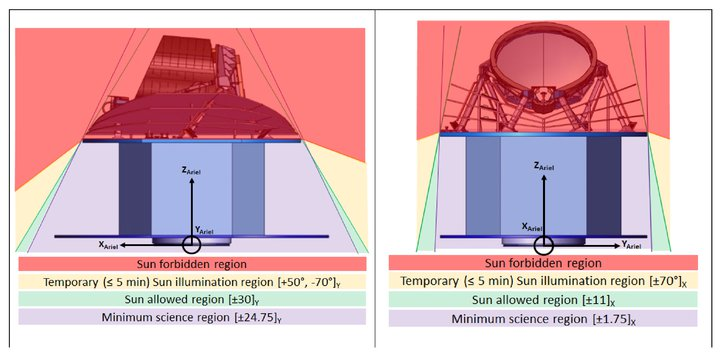
\includegraphics[width=.9\textwidth]{sun no touch.jpg}
    \caption{Illustration of the Sun allowed region (green) in the XZAriel plane (left, showing associated rotations around YAriel) and YZAriel plane (right, showing associated roatations around XAriel) \protect\cite{salvignol2024ariel}.}
    \label{fig:6}
\end{figure}

During operations, the spacecraft maintains a constrained field of regard but is capable of a full 360-degree rotation around its z-axis for optimal target observations. Specific attitude control strategies around the x- and y-axes allow for extended observations of single targets without the need for spacecraft slewing \cite{salvignol2024ariel}.

\subsubsection{Attitude and Autonomy} \label{sec:2.1.3}

The nominal mission lifetime is set at four years, with a possible extension to six years based on performance and operational requirements \cite{salvignol2024ariel}. Mission operations will be conducted through two primary centres:

\begin{itemize}
    \item[-] The \textbf{Mission Operations Centre (MOC)} at ESA's European Space Operations Centre (ESOC), responsible for spacecraft operations and telemetry management \cite{salvignol2024ariel}.
    \item[-] The \textbf{Science Ground Segment (SGS)}, which includes the \textbf{Science Operations Center (SOC)} at ESA's European Space Astronomy Centre (ESAC), and the \textbf{Instrument Operations and Science Data Centre (IOSDC)}, managed by the Ariel Mission Consortium (AMC) \cite{salvignol2024ariel}
\end{itemize}

Due to limited ground station contact periods, Ariel is designed to operate autonomously for at least six days at a time. The \textbf{Attitude and Orbit Control System (AOCS)} autonomously adjusts the spacecraft's orientation to meet the pointing requirements. Attitude adjustments are pre-planned and uploaded in advance, allowing for the 6 days of autonomous operations for onboard manoeuvres and payload configuration commands \cite{salvignol2024ariel}.
These adjustments are executed through ground-commanded attitudes, uplinked target quaternions, or pre-computed attitude profiles from ground control \cite{salvignol2024ariel}.
Autonomous control is critical for maintaining operational integrity, particularly for avoiding Sun exclusion and restricted zones (see Figure \ref{fig:6}). If the AOCS inadvertently directs the spacecraft toward an unsafe position, the onboard Fault Detection, Isolation, and Recovery (FDIR) system prevents dangerous attitudes, ensuring spacecraft safety \cite{salvignol2024ariel}.

\subsection{Observation Strategy} \label{sec:2.2}

Variations in the measured signal from spatially unresolved observations of an exoplanet at different points in its orbit around its host star provide insights into the planet's
atmospheric spectrum and phase-curve modulation. Since both the star and the exoplanet are observed simultaneously, the exoplanet's signal can be isolated by comparing measurements taken at different orbital positions \cite{salvignol2024ariel}.

The Ariel mission observational strategy prioritises continuous phase-curve monitoring, even when multiple orbits are needed. Observations begin and end with the secondary eclipse, which serves as a reference point for the phase-curve measurements.
To maintain precise timing, a margin of 7\% of the orbital period is included before and after the eclipse, minimising the uncertainty in eccentricity (e) to a maximum of 0.1 \cite{salvignol2024ariel}.

Three key observation types are used to analyse different aspects of the exoplanetary atmosphere:

\begin{itemize}
    \item[-] \textbf{Emission/Reflection Spectroscopy During Eclipse/Occultation:} By comparing observations taken in and out of occultation, the planet's dayside spectrum can be determined \cite{salvignol2024ariel}.
    \item[-] \textbf{Transmission Spectroscopy During Transit:} Absorption features in the exoplanet's atmosphere are measured by analysing differences between in-transit and out-of-transit measurements \cite{salvignol2024ariel}.
    \item[-] \textbf{Phase Variation Analysis:} Monitoring changes in the planet's visible hemisphere throughout its orbit reveals insights into energy redistribution and atmospheric dynamics by detecting subtle differences between observations at various orbital phases \cite{salvignol2024ariel}.
\end{itemize}

\begin{table}[H]
    \centering
    \caption{The study of variability through multi-epoch phase curves will be limited to one or two selected planets, such as HD 189733b, with plans to gather three phase-curves for these targets. This comprehensive approach aims to provide a deeper understanding of the atmospheric dynamics and characteristics of the observed exoplanets \protect\cite{charnay2021phasecurve}.}
    \label{tab:3}
    \resizebox{.8\textwidth}{!}{%
    \begin{tabular}{|l|c|c|c|c|}
    \hline
    \textbf{Planet} &
      \textbf{\begin{tabular}[c]{@{}c@{}}Period\\ (days)\end{tabular}} &
      \textbf{\begin{tabular}[c]{@{}c@{}}Orbits Required\\ (SNR $>$ 10)\end{tabular}} &
      \textbf{\begin{tabular}[c]{@{}c@{}}SNR\\ (Thermal Emission)\end{tabular}} &
      \textbf{\begin{tabular}[c]{@{}c@{}}SNR\\ (Reflected Light)\end{tabular}} \\ \hline
    GJ 1214b   & 1.58 & 11     & 1.0 & 0.3 \\ \hline
    K2-266b    & 0.66 & 11     & 1.1 & 0.5 \\ \hline
    55 Cnc e   & 0.74 & 10     & 0.3 & 0.3 \\ \hline
    GJ 436b    & 2.64 & 15     & 2.0 & 0.9 \\ \hline
    GJ 3470b   & 3.34 & 10     & 0.4 & 0.6 \\ \hline
    HD 189733b & 2.22 & 1 or 3 & 5.2 & 3.0 \\ \hline
    HD 209458b & 3.52 & 1 or 3 & 6.1 & 2.3 \\ \hline
    XO-6b      & 3.77 & 10     & 7.6 & 3.5 \\ \hline
    WASP-77Ab  & 1.36 & 10     & 6.1 & 3.5 \\ \hline
    KELT-7b    & 2.73 & 10     & 5.3 & 2.8 \\ \hline
    WASP-74b   & 2.14 & 9      & 7.6 & 3.4 \\ \hline
    XO-3b      & 3.19 & 9      & 5.1 & 3.5 \\ \hline
    WASP-82b   & 2.71 & 7      & 8.8 & 3.0 \\ \hline
    WASP-14b   & 2.24 & 7      & 5.1 & 2.3 \\ \hline
    KELT-O14b  & 1.71 & 7      & 1.1 & 3.9 \\ \hline
    \end{tabular}%
    }
\end{table}

Table \ref{tab:3} summarises known planets from the phase-curve target list, including the number of orbits required to reach a signal-to-noise ratio (SNR) greater than 10. For thermal emission,
we report the highest SNR value between the different photometric channels, assuming a Bond albedo of A$_B$ = 0.3 for planets with T$_p$ $<$ 700 K and A$_B$ = 0.1 for planets with T$_p$ $>$ 700 K \cite{salvignol2024ariel}. 
For reflected light curves, the SNR is calculated by integrating flux over the 0.5 to 1.1 $\mu$m wavelength range, assuming a geometric albedo equal to the Bond albedo. The geometric albedo represents the ratio of a planet's observed brightness (as seen from the light source) to that of an idealised,
fully reflecting, diffusively scattering disc with the same cross-section \cite{salvignol2024ariel}.

\subsection{Operational Phases} \label{sec:2.3}

Following launch, Ariel will undergo a transfer phase of approximately 1 month before reaching the final L2 orbit. The launcher will place the spacecraft on a direct transfer trajectory, requiring three planned control manoeuvres \cite{salvignol2024ariel}:

\begin{itemize}
    \item[-] The first manoeuvre will occur within 1 day after separation from the launcher, but no later than 2 days.
    \item[-] No additional insertion manoeuvre is required.
    \item[-] A six-month commissioning and calibration phase following launcher separation, including 1 month for transfer operations and 5 months of calibration at L2.
\end{itemize}

\begin{figure}[H]
    \centering
    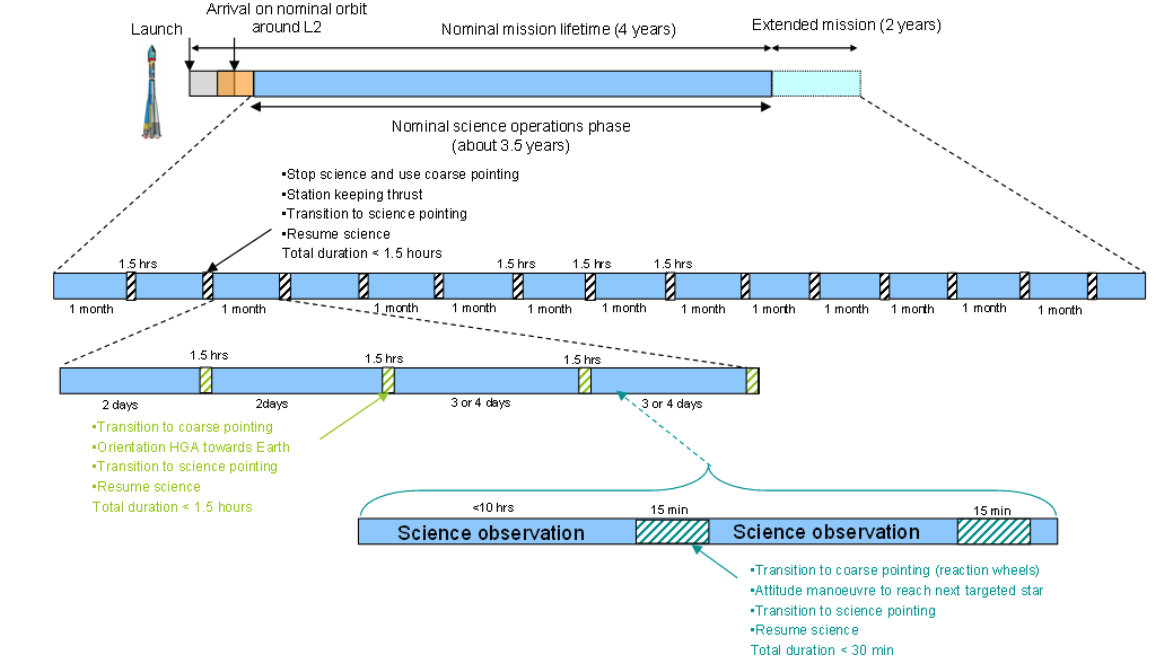
\includegraphics[width=.9\textwidth]{science interruptions.png}
    \caption{\centering Overall Science operation plan and interruptions \protect\cite{salvignol2024ariel}.}
    \label{fig:7}
\end{figure}

Once in the L2 orbit, the spacecraft maintains high availability for scientific observations with only minimal interruptions (see Figure \ref{fig:7}) \cite{salvignol2024ariel}:

\begin{itemize}
    \item[-] \textbf{Station-Keeping manoeuvres:} Conducted every 28 days, requiring less than 2 hours.
    \item[-] \textbf{Data Transmission:} Performed every 2-4 days, the spacecraft reorients its high-gain antenna toward Earth to transmit science data, requiring less than 1.5 hours.
    \item[-] \textbf{Target Transition manoeuvres:} Between successive observations, pointing adjustments and stability convergence require less than 20 minutes.
\end{itemize}

Typical Science observation slots last on average of 7.7 hours, with a maximum duration of up to 3 days per target \cite{salvignol2024ariel}.
Inaction slots are inevitable for the Ariel mission, but through simulation it has been demonstrated that 85\%-90\% of the mission lifetime is available for Science observations, including extra observations of target exoplanets, observations of backup targets,
or using the time for ancillary science (see Figure \ref{fig:8}) \cite{arielstudyreport}.

\begin{SCfigure}[50][ht]
    \centering
    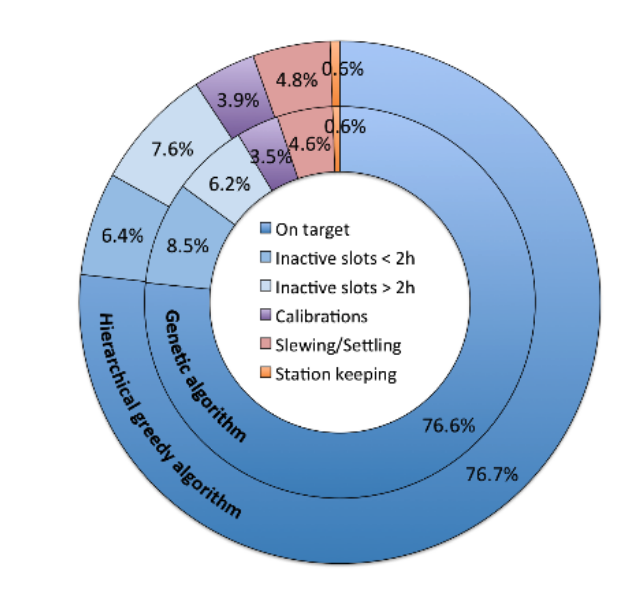
\includegraphics[width=.6\textwidth]{distribution ariel.png}
    \caption{Distribution of the mission lifetime between different operations considered in the Ariel mission planning of the MRS target list. Inner and outer ring charts correspond to the genetic and hierarchical greedy algorithms, respectively. More than
    85-90\% of the time can be used for MRS (on targets time), ancillary science targets (inactive slots), or science calibration observations \protect\cite{arielstudyreport}.}
    \label{fig:8}
\end{SCfigure}

\newpage

\section{Scientific Objectives} \label{sec:3}

\subsection{Past Exoplanet Characterisation Efforts} \label{sec:3.1}

Nasa's Kepler, K2, and TESS missions, alongside ESA's Cheops and PLATO, use visible light to find exoplanets by detecting their transits or measuring their sizes after discovery through radial velocity \cite{ARIEL_M4_Proposal}.
These missions have already found thousands of exoplanets, especially around bright stars, and many more will be discovered in the coming years. The next big step is measuring and studying these planets' atmospheres using infrared (IR) spectroscopy, which can reveal their chemical composition.
However, none of these missions are designed for that, most taking measurements in visible light \cite{platofact,keplerfact} \cite[p.8]{tessfact}, with Cheops the closest at near-infrared \cite[p.4]{fortier2024cheops}.
ESA's Ariel will be the first mission fully dedicated to analysing the atmospheres of hundreds of exoplanets using IR spectroscopy, helping scientists understand their makeup and temperature, expanding our knowledge of planets beyond the Solar System \cite{salvignol2024ariel,ARIEL_M4_Proposal}.

\subsection{Criteria for Exoplanet Selection} \label{sec:3.2}

For the selected sample of observed exoplanets to be statistically significant and representative, it must be both large and diverse \cite{zingales2018ariel}.
The planets must therefore be selected in accordance with various criteria; the sample must contain both gaseous and rocky planets across a range of temperatures, and the host stars must also be of
different spectral types and metallicity. A correspondingly large number of planets covering the widest possible spectrum can be sourced and selected from exoplanets discovered by previous missions, such as
the Kepler Space Mission \cite{zingales2018ariel} and the Transiting Exoplanet Survey Satellite (TESS) \cite{arielTESScandidates}.

The Ariel mission will focus primarily on planets with an orbital period less than 50 days, typically corresponding to warmer planets (see Figure \ref{fig:9}). 

\begin{figure}[H]
    \centering
    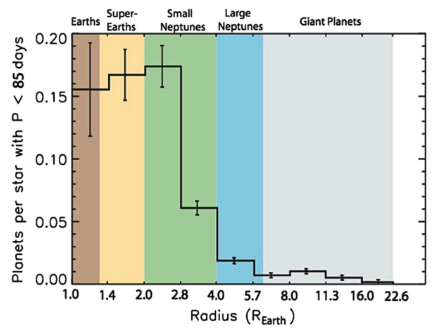
\includegraphics[width=.75\textwidth]{planet w small orbits.png}
    \caption{Average number of planets per star and per size bin with an orbital period shorter than 85 days orbiting around F, G, K stars \protect\cite{zingales2018ariel}}
    \label{fig:9}
\end{figure}

\subsection{Ariel Tier List System for Observational Prioritisation} \label{sec:3.3}

To maximise the science return of Ariel, a three-tiered system has been devised where the three different samples are observed at optimised spectral resolutions, wavelength intervals,
and SNR \cite{salvignol2024ariel}. An additional fourth tier has been planned for additional time to observe the phase-curves of Tier 3 planets \cite{arielstudyreport} (see Table \ref{tab:1}, Table \ref{tab:2}).

\begin{table}[H]
    \caption{Table of the Ariel tiers presented, with percentage of dedicated mission lifetime and requirements for each tier shown \protect\cite{arielstudyreport,salvignol2024ariel}.}
    \centering
    \label{tab:1}
    \resizebox{\textwidth}{!}{        
        \begin{threeparttable}
            \renewcommand{\arraystretch}{1.55}
            \begin{tabular}{|l@{\hskip 15pt}|l|}
            \hline
            Survey ($\sim$30\%)\protect\tnote{**} &
            \begin{tabular}[c]{@{}l@{}}Low spectral resolution observations (R $\geq$ 10 across all channels) of a large sample\\ of planets in the VIS-IR, with SNR $\geq$ 7\end{tabular} \\ \hline
            Deep ($\sim$60\%)\protect\tnote{**} &
            \begin{tabular}[c]{@{}l@{}}Intermediate spectral resolution observations (R $>$ 50 in AIRS channel 0 and R $>$ 15 \\ in AIRS channel 1) of a sub-sample in the VIS-IR\end{tabular} \\ \hline
            Benchmark ($\sim$6\%)\protect\tnote{**}    & Very best planets, re-observed multiple times with all techniques; full spectral resolution \\ \hline
            Phase Curves ($\sim$4\%)\protect\tnote{**} & Multiple-band photometry/spectroscopy with SNR $\geq$ 4; spatial variability                     \\ \hline
            \end{tabular}%
            \begin{tablenotes}
                \footnotesize
                \item[**] \textit{\% correspond to mission lifetime spent at each tier}
            \end{tablenotes}
        \end{threeparttable}
    }
\end{table}

\begin{table}[H]
    \caption{The total science time is $\sim$24 800 hr over the primary 4-year mission lifetime. Table of mission time required to achieve different observation goals. Note that for some bright targets (e.g. HD 209458b) Tier 2 or Tier 3 
    resolutions would be reached in a single observation \protect\cite{arielstudyreport}.}
    \centering
    \label{tab:2}
    \resizebox{.8\textwidth}{!}{%
        \begin{tabular}{lcc}
        \multicolumn{3}{c}{Mission Time Required to Achieve Different Observation Goals}                                                                       \\ \hline
        \textbf{Number of Planets} &
        \textbf{Observation Requirement} &
        \textbf{Required Science Time (hr)} \\ \hline
        1000 & Achieve Tier 1 resolutions                                                               & $\sim$10 600 \\ \hline
        \begin{tabular}[c]{@{}l@{}}400\\ \\ 500\\ 600\end{tabular} &
        \begin{tabular}[c]{@{}c@{}}Increase resolution from Tier 1\\ to Tier 2\end{tabular} &
        \begin{tabular}[c]{@{}c@{}}$\sim$3100\\ \\ $\sim$6000\\ $\sim$10 500\end{tabular} \\ \hline
        \begin{tabular}[c]{@{}l@{}}200\\ \\ 300\\ 400\end{tabular} &
        \begin{tabular}[c]{@{}c@{}}Achieve Tier 1 resolutions in the\\ second method\end{tabular} &
        \begin{tabular}[c]{@{}c@{}}$\sim$1400\\ \\ $\sim$2500\\ $\sim$4200\end{tabular} \\ \hline
        50   & \begin{tabular}[c]{@{}c@{}}Tier 3 (five repeated observations\\ per planet)\end{tabular} & $\sim$1700   \\ \hline
        ...  & Tier 4 (additional science time)                                                         & $\sim$2300   \\ \hline
        \end{tabular}%
    }
\end{table}

The orbit and attitude limits of the spacecraft must also be considered for measurements during scheduling in order to maximise the science time. Figure \ref{fig:1} illustrates the distribution of targets in right ascension and declination (equatorial) coordinates for the fraction of the year
that each region of the sky is visible within Ariel's proposed orbit at the Sun-Earth Lagrangian point L2. Any direction is observable for at least $\sim$30\% of the year \cite{zingales2018ariel,morales2022ariel}.

\begin{figure}[H]
    \centering
    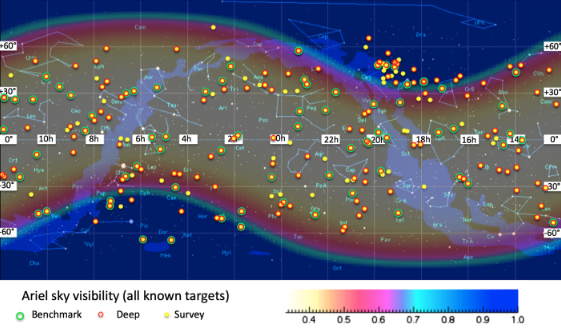
\includegraphics[width=.9\textwidth]{ariel target map.png}
    \caption{A plot illustrating the fraction of the year for which a given location in the sky (in equatorial coordinates) is visible to Ariel, as seen from a representative operational
    orbit of Ariel at L2. \textbf{Yellow} dots: planets observed in Tier 1. \textbf{Red} dots: planets observed in Tier 2. \textbf{Green} dots: planets observed in Tier 3. \protect\cite{zingales2018ariel} The background colour levels represent the fraction of the year for which
    region of the sky is visible for Ariel \cite{morales2022ariel}.}
    \label{fig:1}
\end{figure}

\subsubsection{Survey (Tier 1)} \label{sec:3.3.1}

Tier 1 observations will help refine orbital and planetary parameters that can then be used to limit or completely remove degeneracies in the interpretation of mass-radius diagrams.
Most giant planets and Neptunes fulfil the Tier 1 criteria set for the science objectives in 1 transit/eclipse, while the smaller planets would require upwards of 6 events (see Figure \ref{fig:3}) \cite{zingales2018ariel}.
Additionally, it will be possible to generate colour-colour and colour-magnitude diagrams, which might lead to the same developments in understanding as the H-R diagram did \cite{edwards2019updated,salvignol2024ariel}.

\begin{figure}[H]
    \centering
    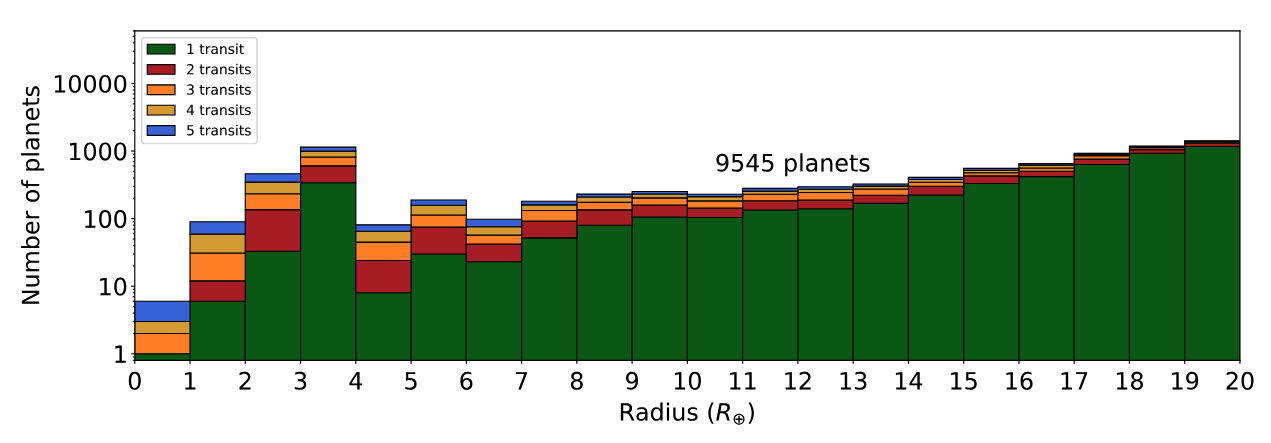
\includegraphics[width=.9\textwidth]{tier 1 transit graph.png}
    \caption{Complete set of Tier 1 planets from the Ariel mission reference population. The final list of Tier 1 planets will include an optimal sub-sample. Different colours indicate the number of transits/eclipses needed to reach
    Tier 1 performances. The planets shown here can achieve the Tier 1 requirements combining the signal of $\leq$ 5 transits/eclipses \protect\cite{zingales2018ariel}.}
    \label{fig:3}
\end{figure}

Tier 1 observations will answer the following questions:

\textbf{"What fraction of planets are covered by clouds?"}\\
This method of observation helps differentiate between planets with clear atmospheres and those of denser cloud cover, as this obscures molecular absorption features typically present in spectra.
Extremely cloudy planets can be identified from low-resolution across a broad wavelength range. This allows scientists to determine whether a planet should continue with higher-resolution spectral classification
(i.e., be included in the Tier 2 sample) or not \cite{salvignol2024ariel}.\\

\textbf{"What fraction of small planets still have hydrogen and helium retained from the protoplanetary disc?"}\\
This question is essential to understand the formation and evolution of super-Earths. Primordial (primary) atmospheres are expected to consist of mainly hydrogen and helium,
reflecting the gaseous composition of the protoplanetary nebula. If an atmosphere is made up of heavier metals, it likely indicates that the atmosphere has evolved, thus resulting in a secondary atmosphere.
The easiest way to differentiate between primary (hydrogen-rich) and secondary (metal-rich) atmospheres is through transmission spectroscopy as the main atmospheric component directly affects atmospheric scale height \cite{salvignol2024ariel}. \\

\textbf{"What is the bulk composition of the terrestrial exoplanets?"}\\
Planetary density provides insight into a planet's interior composition, but this measurement alone may lead to non-unique interpretations. Analysing composition of the upper atmosphere in transiting planets will help reveal the degree 
of composition separation between the planet's atmosphere and interior. This approach reduces uncertainties in the presence and mass of the atmosphere, resolving potential doubtfulness in understanding the planet's overall makeup \cite{salvignol2024ariel}. \\

\textbf{"What is the energy balance of the planet?"}\\
Through analysis of eclipse measurements in optical and infrared wavelengths scientists can determine overall temperature and albedo (the fraction of diffracted sunlight) of the planet. These measurements
help estimate the planetary energy balance and whether the planet has an internal heat source \cite{salvignol2024ariel}.

\begin{figure}[H]
    \centering
    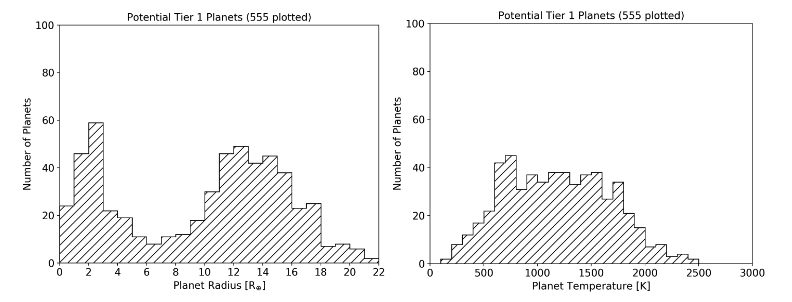
\includegraphics[width=.9\textwidth]{tier 1 radius and temp plots.png}
    \caption{Currently known Ariel planetary candidates plotted as a function of planetary radius (left) and planetary temperature (right) \protect\cite{arielstudyreport}.}
    \label{fig:2}
\end{figure}

Ariel's Tier 1 survey mode will allow for fast and comprehensive initial assessments of planets, accommodating informed decisions when deciding what planets to further examine during Tier 2 and Tier 3 observations \cite{salvignol2024ariel}.
Observing Figure \ref{fig:2}, illustrating the distribution of potential Tier 1 targets for the Ariel mission as functions of planetary radius and temperature, it can be seen that over 500 currently known planets already comply with Tier 1 requirements \cite{arielstudyreport,edwards2019updated}.

\subsubsection{Deep (Tier 2)} \label{sec:3.3.2}

A key objective of the Ariel mission is to investigate whether a correlation exists between a planet's chemical composition and fundamental properties such as mass, radius, and temperature. To achieve this, Tier 2 observations will conduct high-resolution spectroscopic measurements with focus on studying both individual
exoplanets and populations. This approach allows detailed examinations of various exoplanetary atmospheric characteristics, including \cite{salvignol2024ariel}:

\begin{itemize}
    \item[-] \textbf{Primary Atmospheric Composition in Smaller Planets:} Identifying the main gases in the atmosphere of smaller exoplanets, which is essential for characterising their atmospheric properties \cite{salvignol2024ariel}.
    \item[-] \textbf{Trace Gas Abundance:} Measuring abundance and concentration of trace gases to determine the type of chemistry happening in the atmosphere, and whether it is in equilibrium of non-equilibrium states \cite{salvignol2024ariel}.
    \item[-] \textbf{Atmospheric Thermal Structure:} Analysing the thermal structure, both vertically and horizontally, of the atmosphere to understand the impact on atmospheric structure and energy distribution \cite{salvignol2024ariel}.
    \item[-] \textbf{Cloud Characteristics:} Examining cloud properties, such as particle size and distribution, to understand their impact on climate and atmospheric dynamics \cite{salvignol2024ariel}.
    \item[-] \textbf{Elemental Composition in Gaseous Planets:} Investigating the elemental makeup of gaseous planets to constrain formation models and enhance the understanding of planetary evolution \cite{salvignol2024ariel}.
\end{itemize}

By integrating these measurements, the Tier 2 Deep Survey observations aim to provide a comprehensive view and understanding of atmospheric characteristics in a broad range of exoplanets, enabling comparisons across different planetary populations and contributing to the advancement of the broader goals of the Ariel mission \cite{salvignol2024ariel}.

\subsubsection{Benchmark (Tier 3)} \label{sec:3.3.3}

The Ariel Tier 3 observations are dedicated to the detailed study of atmospheric variability in a select group of exoplanets, known as benchmark planets. A portion of these planets, particularly those orbiting very bright stars, will be observed multiple times over an extended time-period to gather essential data. The key objectives of these observations include \cite{salvignol2024ariel}:

\begin{itemize}
    \item[-] \textbf{Primary Knowledge of Planetary Chemistry and Dynamics:} Examining the chemical processes within exoplanet atmospheres to better understand their composition and behaviour \cite{salvignol2024ariel}.
    \item[-] \textbf{Elemental Composition Analysis:} Investigating the distribution of elements, both within the atmosphere and on the planet's surface, to gain insights into formation and evolutionary history \cite{salvignol2024ariel}.
    \item[-] \textbf{Weather Patterns and Atmospheric Variability:} tracking spatial and temporal changes in atmospheric conditions, including temperature variations, cloud coverage, and atmospheric circulation dynamics, to gain insight into the weather systems of exoplanets \cite{salvignol2024ariel}.
\end{itemize}

Benchmark planets are identified as ideal candidates for phase-curve spectroscopic measurements due to their high spectral resolution and strong signal-to-noise ratios (SNR), allowing for meaningful observations in just one or two observations.
The focus will be on "weather planets", selected for their potential to showcase significant atmospheric changes over time \cite{salvignol2024ariel}.

By conducting repeated observations, Ariel Tier 3 observations aim to capture the temporal evolution of exoplanetary atmospheres, revealing essential insights into cloud formation, atmospheric circulation, and climate dynamics on exoplanets \cite{salvignol2024ariel}.
Figure \ref{fig:4} shows a possible MRS (Mission Reference Sample) with all three tiers discussed (Survey, Deep, Benchmark) nested together, optimised to yield maximum number of targets. 

\begin{figure}[H]
    \centering
    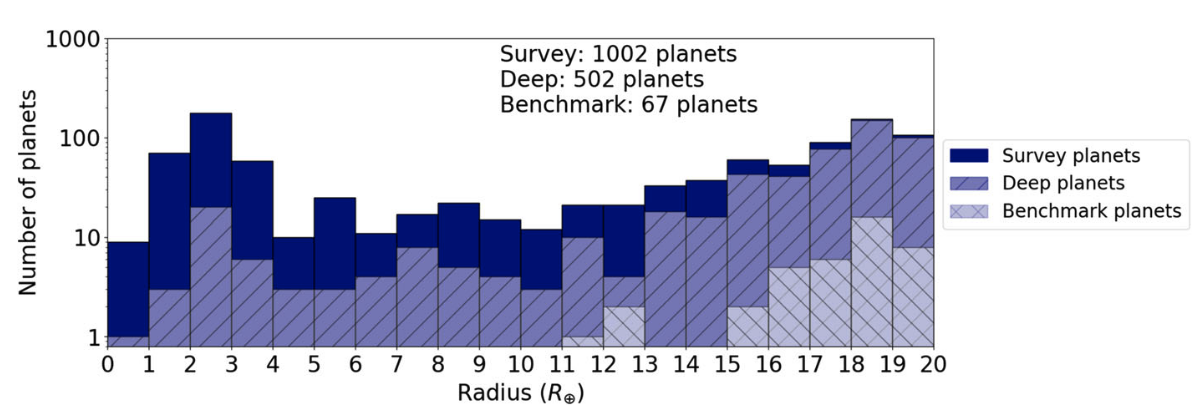
\includegraphics[width=.9\textwidth]{comparison tiers.png}
    \caption{Overview of the Ariel MRS (Mission Reference Sample), comparing the number of planets observable in the three tiers during the mission lifetime \protect\cite{zingales2018ariel}.}
    \label{fig:4}
\end{figure}

\subsubsection{Phase Curves (Tier 4)} \label{sec:3.3.4}

To gain deeper insights on targets of special interest, bespoke observations are conducted to study their spatial variability and gather detailed information on planetary chemistry and atmospheric dynamics. 
Tier 4 planets will be selected from Tier 3 Benchmark planets based on their potential to exhibit significant atmospheric variability (see Figure \ref{fig:5}) \cite{edwards2022ariel}.
A key method used in analysis is through observing planetary phase curves, which answers several fundamental questions \cite{arielstudyreport}:

\begin{itemize}
    \item[-] \textbf{Factors Influencing Atmospheric Heat Redistribution:} This investigation aims to identify how factors such as stellar irradiation, planetary radius, metallicity (the abundance of elements heavier than hydrogen and helium), and orbital eccentricity
    impact atmospheric heat redistribution. By measuring dayside and nightside emissions, and also phase offsets, researchers can gain details about circulation regimes, radiative timescales, wind speeds, and the role of nightside clouds \cite{arielstudyreport}.
    \item[-] \textbf{Variations in Atmospheric Composition and Thermal Structure:} This analysis focuses on how the chemical composition and thermal structure of strongly irradiated planets change from the dayside to the nightside. Atmospheric circulation is expected to smooth
    out variations, leading to chemical disequilibrium, and potential temperature fluctuations and thermal variations on the dayside \cite{arielstudyreport}.
    \item[-] \textbf{Atmospheric Composition of Low-Mass Planets:} A key objective is determining the atmospheric composition and metallicity of low-mass exoplanets. It is predicted that planets with higher atmospheric metallicity will exhibit greater heat redistribution and higher
    amplitude phase curves, allowing for independent measurements of atmospheric metallicity \cite{arielstudyreport}.
    \item[-] \textbf{Albedo of Exoplanets:} This question investigates the nature of tiny particles present in exoplanetary atmospheres, particularly condensate clouds and photochemical hazes. Measuring the planet's albedo is important for understanding its temperature balance.
    Since temperature variations can influence the albedo, understanding this relationship can provide valuable insights into exoplanet climate and atmospheric conditions \cite{arielstudyreport}.
\end{itemize}

By integrating these observations, researchers can develop a more comprehensive understanding of exoplanetary atmospheres, their dynamics, chemistry, and climate, further advancing the field of comparative planetology.

\begin{SCfigure}[50][hb]
    \centering
    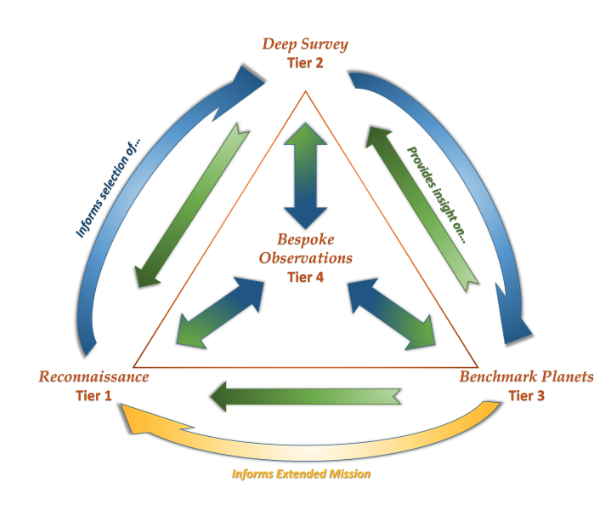
\includegraphics[width=.55\textwidth]{tiers ariel.png}
    \caption{Schematic diagram of Ariel's 4-Tier ecosystem. Tier 1 will provide the base for selecting Tier 2 planets, which in turn inform the selection of Tier 3 targets. The planets in each Tier will give deeper insight into the nature of the planets in preceding Tiers. This interdependence among Tiers means that the
    scientific value of the data collected by Ariel will grow over time. Tier 4 observations will benefit from the insight gained by the planetary populations of the other Tiers and will in turn provide better understanding of their atmospheric behaviour \protect\cite[p.40]{arielstudyreport}.}
    \label{fig:5}
\end{SCfigure}

\subsection{The Scientific Reasoning for Studying Hot Exoplanets} \label{sec:3.4}

Hot planets provide a unique opportunity to study their elemental and chemical composition because their atmospheres lack cold traps that would otherwise condense key molecules, like H$_2$O NH$_3$, CH$_4$, SiO, CO$_2$, CO, and, at high temperatures, metallic compounds such as TiO, VO, and CrH \cite{ARIEL_M4_Proposal} \cite[p.135]{tinetti2018chemical}.
Understanding these hot planets is crucial for building a broad foundation before shifting the focus to cooler planets. Moreover, many of the exoplanets discovered so far, or expected to be found, are in close orbits around their stars, making them naturally hot. Their short orbital periods make them ideal candidates for transit and eclipse spectroscopy, allowing detailed
atmospheric studies. While the ultimate goal is to characterise a wide range of exoplanets, including potentially habitable ones, Ariel will serve as a crucial stepping stone, paving the way for even more advanced future missions \cite{ARIEL_M4_Proposal}.

\newpage

\section{Spacecraft Overview} \label{sec:4}

The Ariel spacecraft is designed to provide a stable, deep-space thermal environment for exoplanet observations. It consists of two main modules: the \textbf{Service Module (SVM)} and the \textbf{Payload Module (PLM)}.
The modular design allows independent construction and testing of each module, optimising integration facility (see Figure \ref{fig:15}) \cite{salvignol2024ariel}.
The SVM houses essential platform subsystems while the PLM houses the scientific instrumentation and optical components \cite{salvignol2024ariel}. The spacecraft is three-axis stabilised and thermally optimised to maintin the PLM at operating temperatures ($<$70 K), shielded from solar
input and spacecraft-generated heat \cite{salvignol2024ariel}

\subsection{Service Module (SVM)} \label{sec:4.1}

\subsubsection{Structure and Thermal Design} \label{sec:4.1.1}

The SVM is constructed with a central cylinder, side cones, shear panels, and top and bottom panels (see Figure \ref{fig:15}). The central cylinder serves as the primary structural element, carrying launch loads and integrating with the launch vehicle adapter at its base. 
The propellant tanks are housed within this structure (see Figure \ref{fig:16}) \cite{morgante2022thermal}.

\begin{figure}[H]
    \centering
    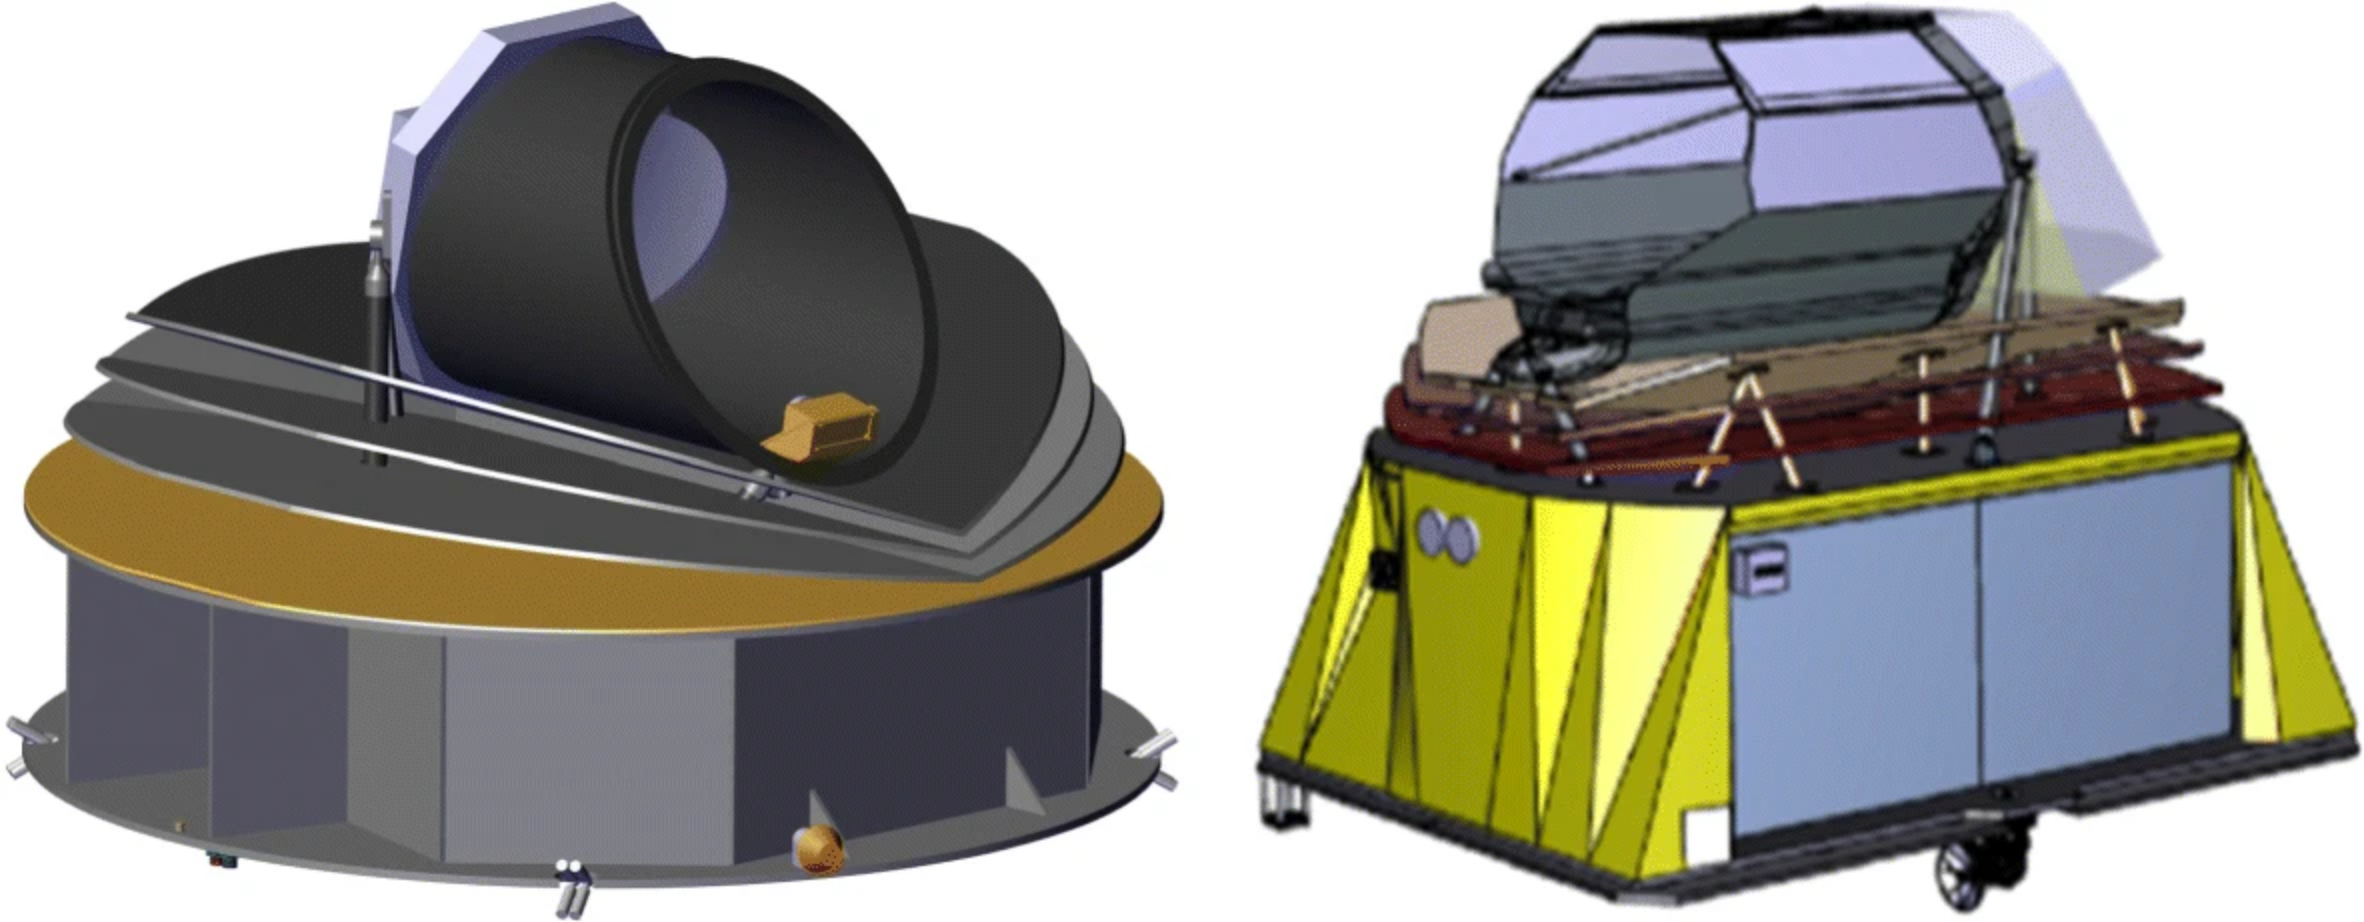
\includegraphics[width=\textwidth]{industrial ariel.png}
    \caption{Industrial S/C designs (courtesy of TAS and ADS) with alternative PLM compared to the Consortium baseline PLM \protect\cite{puig2018phase}.}
    \label{fig:15}
\end{figure}

To ensure thermal stability, the SVM maintains a controlled operational temperature of approximately 20$^{\circ}$C thorugh a combination of heaters and radiator panels, which dissipate excess hear toward deep space. This design ensures that no SVM components directly radiate toward
the PLM, preventing thermal contamination \cite{arielassessreport,morgante2022thermal}.

\begin{figure}[H]
    \centering
    \begin{minipage}{.4\textwidth}
        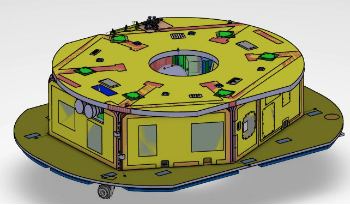
\includegraphics[width=\linewidth]{ariel svm1.png}
        \vfill
        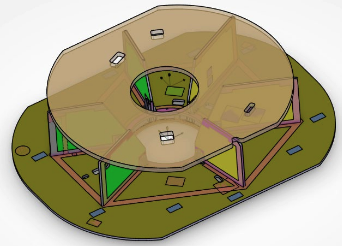
\includegraphics[width=\linewidth]{ariel core1.png}
    \end{minipage}
    \hspace{-.5em}
    \begin{minipage}{.4\textwidth}
        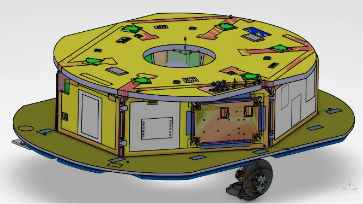
\includegraphics[width=\linewidth]{ariel svm2.png}
        \vfill
        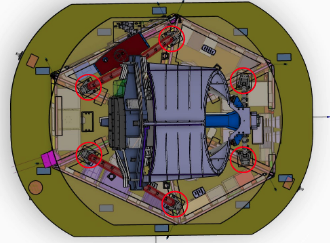
\includegraphics[width=\linewidth]{ariel core2.png}
    \end{minipage}
    \caption{\centering Ariel SVM (top) and core (bottom) structure overview \protect\cite{salvignol2024ariel}}
    \label{fig:16}
\end{figure}

\subsubsection{Attitude and Orbital Control Subsystem (AOCS)} \label{sec:4.1.2}

The AOCS ensures precise spacecraft orientation and telescope stability. It operates in two modes \cite{arielassessreport}:

\begin{itemize}
    \item[-] \textbf{Coarse Pointing Mode:} Utilises star trackers and reaction wheels to slew between targets.
    \item[-] \textbf{Fine Pointing Mode:} Engages the Fine Guidance System (FGS) within the PLM for highly accurate telescope alignment during observations.
\end{itemize}

\subsubsection{Propulsion System} \label{sec:4.1.3}

The propulsion system is a mono-propellant hydrazine-based system, incorporation 1-20 N thrusters. These thrusters support reaction wheel desaturation, safe-mode operations, and orbital correction manoeuvres \cite{arielassessreport}.

\subsubsection{Electrical and Communication System} \label{sec:4.1.4}

The spacecraft is powered by fixed solar panels mounted on the floor of the SVM, eliminating the need for deployable solar arrays. Since Ariel's orbit is eclipse-free, onboard batteries and primarily needed for launch and orbital manoeuvres \cite{arielassessreport}.

Communication is facilitated through two sets of antennas \cite{arielassessreport}:

\begin{itemize}
    \item[-] \textbf{Low Gain Antennas (LGA):} Used for recovery scenarios and low-data-rate uplinks.
    \item[-] \textbf{Medium Gain Antennas (MGA):} Used for high-data-rate uplinks, ensuring seamless transmission of science data.
\end{itemize}

Weekly ground contact is planned for 14 hours, distributed over three sessions of 4-6 hours each. The onboard memory is designed to accommodate continuous science operations, with sufficient storage
capacity to prevent data loss in the event of a missed ground contact \cite{arielassessreport}.

\subsection{Payload Module (PLM)} \label{sec:4.2}

\subsubsection{Structure and Thermal Control} \label{sec:4.2.1}

The PLM consists of a thermal shield assembly and an optical bench. The thermal shield employs a three-layer V-groove configuration to minimise heat transfer from the SVM, maintaing the PLM at optimal operational temperatures (see Figure \ref{fig:16}) \cite{salvignol2024ariel,morgante2022thermal}.
The PLM is mounted on the SVM via three Glass-Fiber Reinforced Polymer (GFRP) bipods, reducing thermal conductivity between the modules \cite{morgante2022thermal}.

The cold and warm components of the PLM are thermally isolated and connected by a cryoharness \cite{arielassessreport,morgante2022thermal,ARIEL_M4_Proposal}. The cold unit, operating at 40 K, houses the spectrometer and FGS, while the warm unit, operating at $\sim$293 K, contains supporting 
electronics and control systems \cite{ARIEL_M4_Proposal}. The telescope instruments are further cooled using a radiator to maintain stability \cite{morgante2022thermal,arielassessreport}.

\subsubsection{Telescope System} \label{sec:4.2.2}

The Ariel telescope is a Cassegrain design, featuring a primary concave mirror (M1) and a secondary convex mirror (M2) (see Figure \ref{fig:17}). At third mirror (M3) collimates the incoming light, directing it along the x-axis to a dichroic beam splitter (D1).
The split beams are then routed to the FGS and AIRS via additional optical elements (see Figure \ref{fig:17}) \cite{ARIEL_M4_Proposal}.

\begin{figure}[hb]
    \centering
    \begin{subfigure}[b]{.49\textwidth}
        \centering
        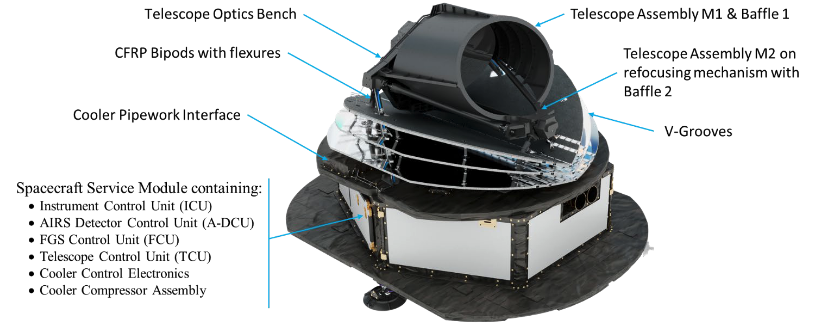
\includegraphics[width=\linewidth]{ariel label1.png}
        \caption{Illustration of the Ariel PLM and SVM}
    \end{subfigure}
    \hfill
    \begin{subfigure}[b]{.49\textwidth}
        \centering
        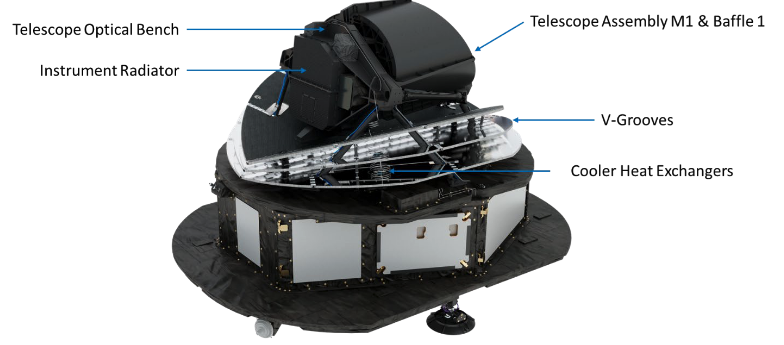
\includegraphics[width=\linewidth]{ariel label2.png}
        \caption{Illustration of the rear of the Ariel PLM}
    \end{subfigure}
    \caption{Illustration of the Ariel spacecraft \protect\cite{salvignol2024ariel}.}
    \label{fig:18}
\end{figure}

The telescope structure is built using silicon carbide (SiC) mirrors mounted on a carbon-fiber frame, providing high stability with minimal thermal expansion \cite{ARIEL_M4_Proposal}.

\subsubsection{Ariel Infrared Spectrometer (AIRS)} \label{sec:4.2.3}

AIRS is the primary scientific instrument of Ariel, designed for spectromscopic analysis of exoplanet atmospheres. It covers a wavelength range of 1.95 - 7.80 $\mu$m, split into two channels:

\begin{itemize}
    \item[-] \textbf{Channel 0 (CH0):} 1.95-3.9 $\mu$m \cite{salvignol2024ariel,ARIEL_M4_Proposal}.
    \item[-] \textbf{Channel 1 (CH1):} 3.9-7.8 $\mu$m \cite{salvignol2024ariel,ARIEL_M4_Proposal}.
\end{itemize}

Each channel contains a spherical mirror that directs light into a common focal plane (see Figure \ref{fig:17}). AIRS achieves a spectral resolving power of 100-200, enabling the detection of key exoplanetary molecules, such as
H$_2$O, CH$_4$, CO, CO$_2$, and NH$_3$ \cite{martignac2022airs,ARIEL_M4_Proposal}.

\begin{figure}[H]
    \centering
    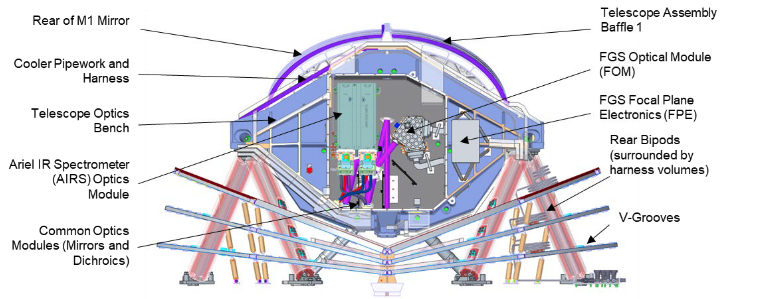
\includegraphics[width=.8\textwidth]{plm.png}
    \caption{\centering Illustration of the accommodation of the Ariel PLM Optical Bench \protect\cite{salvignol2024ariel}.}
    \label{fig:17}
\end{figure}

AIRS is comprised of four main components (see Figure \ref{fig:18}, Figure \ref{fig:17}):

\begin{itemize}
    \item[-] AIRS Optical Bench (AIRS-OB)
    \item[-] AIRS Focal Plane Assembly (AIRS-FPA-CH0 and AIRS-FPA-CH1)
    \item[-] AIRS Cold Front-End Electronics (AIRS-CFEE-Ch0 and AIRS-CFEE-CH1)
    \item[-] AIRS Detector Control Unit (A-DCU) \textit{(located on the warm side of the PLM)}
\end{itemize}

\subsubsection{Fine Guidance System (FGS)} \label{sec:4.2.4}

The FGS is reponsible for precise spacecraft alignment and also provides photometric data. It measures starlight variations to refine the pointing accuracy, feeding information to the AOCS. The FGS
consists of three photometric channels \cite{martignac2022airs,ARIEL_M4_Proposal}:

\begin{itemize}
    \item[-] \textbf{VISPhot:} 0.5-0.6 $\mu$m \cite{salvignol2024ariel}.
    \item[-] \textbf{FGS1:} 0.6-0.8 $\mu$m \cite{salvignol2024ariel}.
    \item[-] \textbf{FGS2:} 0.8-1.10 $\mu$m \cite{salvignol2024ariel}.
\end{itemize}

Additionally, the low-resolution spectrometer covers 1.10-1.95 $\mu$m for supplementary data collection \cite{ARIEL_M4_Proposal,salvignol2024ariel}. The FGS operates at $\sim$50 K and is mounted on the optical bench alongside the AIRS instrument (see Figure \ref{fig:17}).
It includes an independent control system located in the SVM, with real-time data processing capabilities and in-orbit reprogramming functionality \cite{ARIEL_M4_Proposal}.

\subsubsection{Analysis and Testing of the PLM} \label{sec:4.2.5}

\paragraph{Surface Charging Analysis} ~\\

In order to reach its operational orbit, the Ariel PLM must pass through several transfer orbits, including a low Earth orbit, a geostationary orbit (GEO), and an orbit around L2, exposing it to radiation and potential surface charging. Key environmental changes at L2
include passage through the Earth's magnetosheath, magnetotail, and direct solar wind (see Figure \ref{fig:11}). This exposure increases the risk of spacecraft charging, which can interfere with critical systems and signals, justifying the need for testing \cite{Michelagnoli_Focardi_Pudney_Renouf_Merola_Noce_Nunez_Dinuzzi_Chiarucci_2024}.

\begin{figure}[ht]
    \centering
    \begin{subfigure}[b]{.45\textwidth}
        \centering
        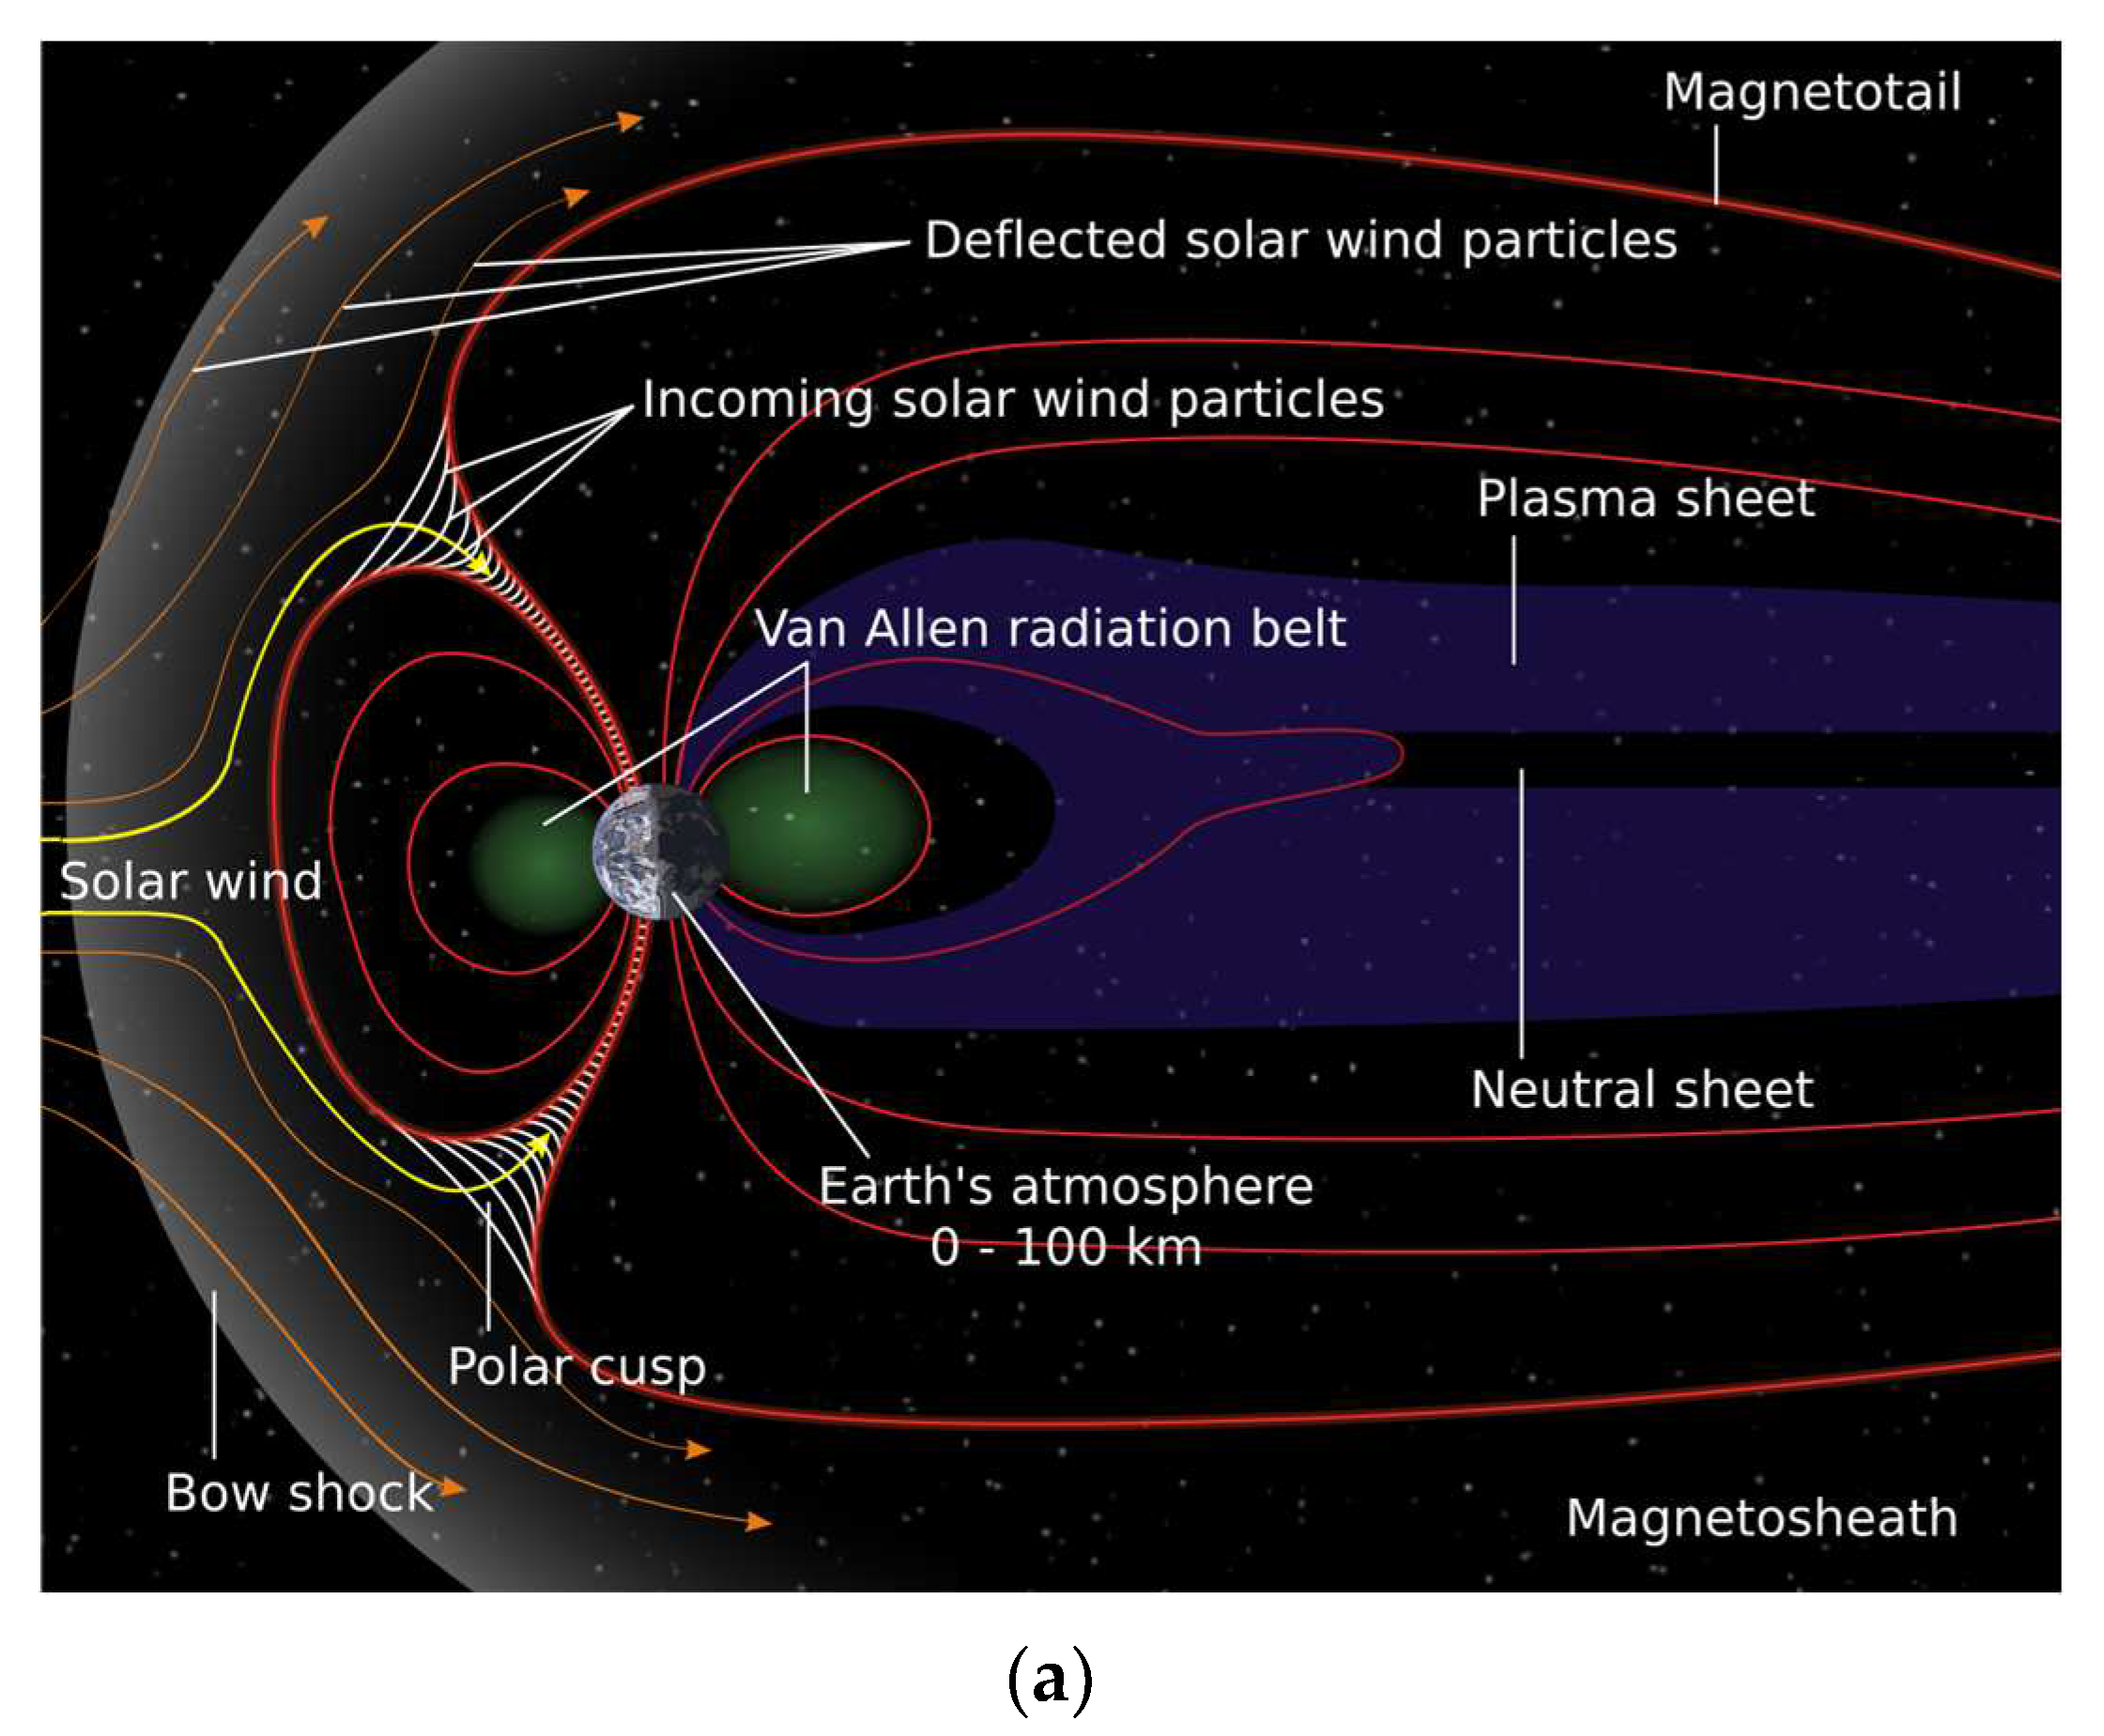
\includegraphics[width=\linewidth]{ariel mag1.png}
    \end{subfigure}
    \hspace{-.5em}
    \begin{subfigure}[b]{.45\textwidth}
        \centering
        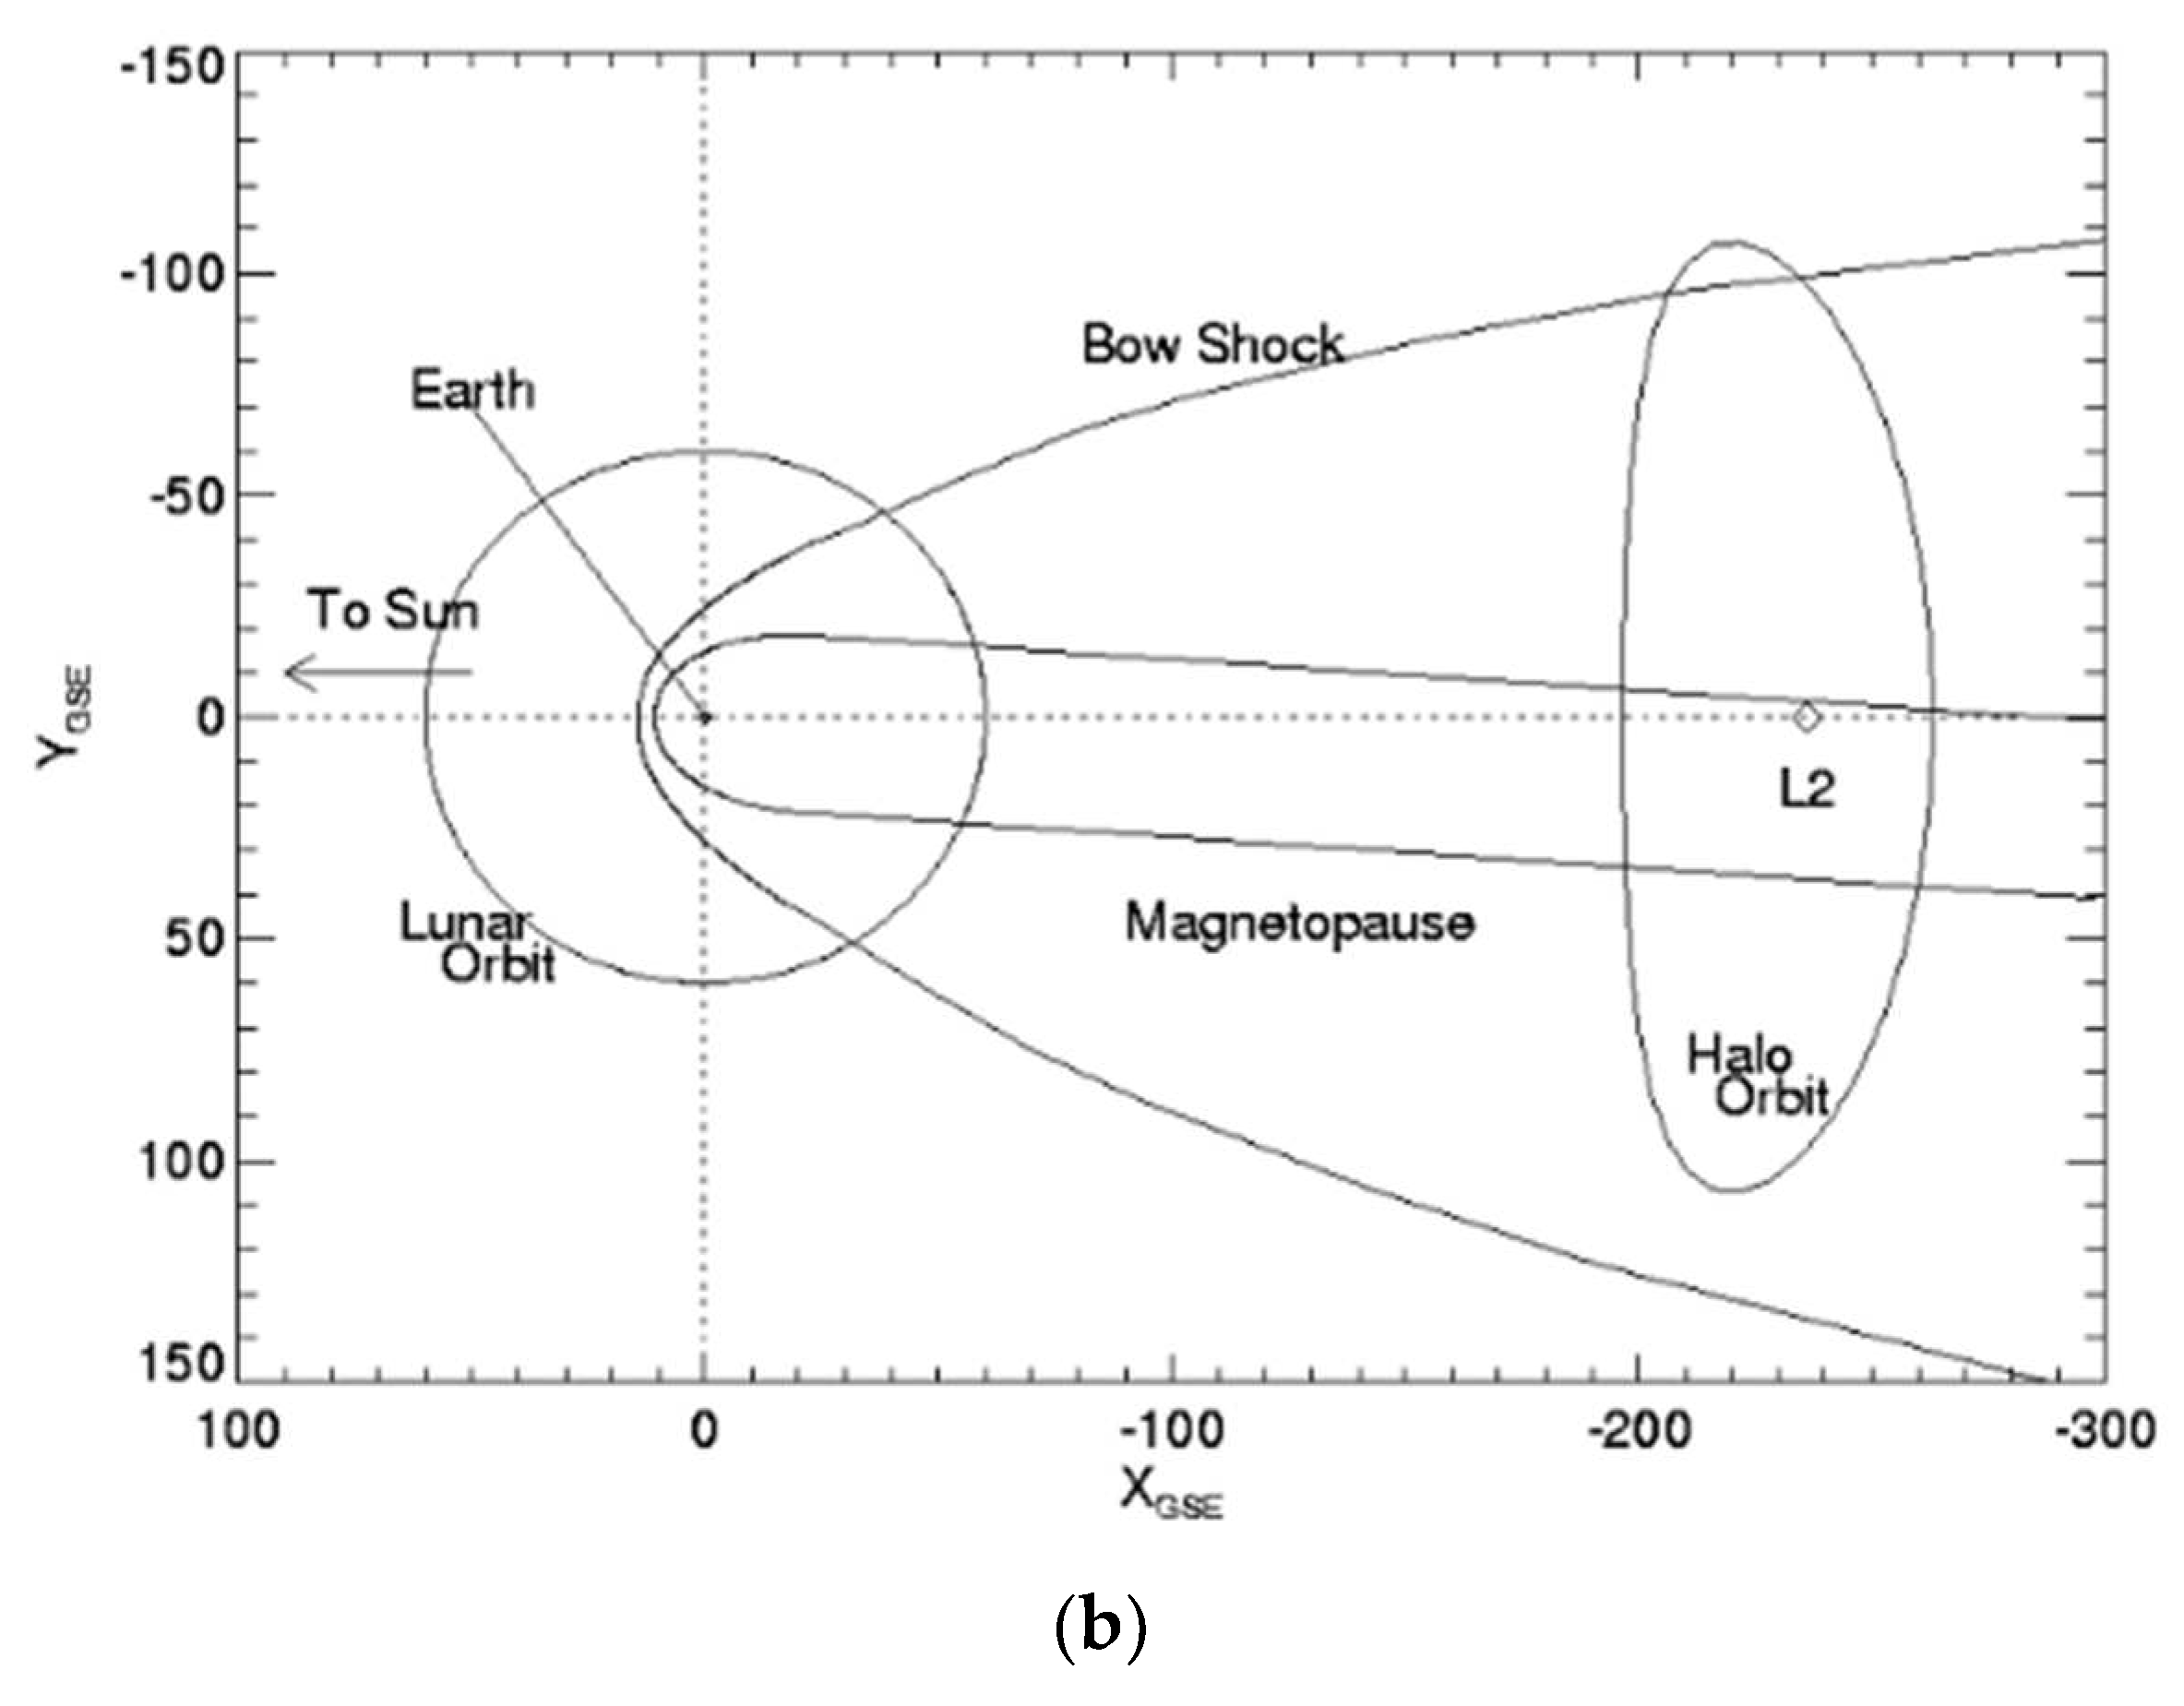
\includegraphics[width=\linewidth]{ariel mag2 simple.png}
    \end{subfigure}
    \caption{(a) Earth-Moon system, magnetotail, magnetopause, bow shock, and halo orbit around L2; (b) Schematic of the simplified structure of Earth's magnetosphere \protect\cite{Michelagnoli_Focardi_Pudney_Renouf_Merola_Noce_Nunez_Dinuzzi_Chiarucci_2024}.}
    \label{fig:11}
\end{figure}

Spacecraft charging occurs when charge accumulates on the exterior (surface charging) or within materials (bulk/deep dielectric charging). The worst-case scenario involved mission failure due to system disruptions. The primary contributors to charging on Ariel are plasma interactions and
solar radiation, with other contributors considered negligible, as electrons pose a higher risk due to their higher velocities \cite{Michelagnoli_Focardi_Pudney_Renouf_Merola_Noce_Nunez_Dinuzzi_Chiarucci_2024}. Secondary effects, such as photoelectric emissions, may influence net charge balance. However, leaning too far in either
direction could damage equipment (see Figure \ref{fig:10}) \cite{Michelagnoli_Focardi_Pudney_Renouf_Merola_Noce_Nunez_Dinuzzi_Chiarucci_2024}. 

\begin{figure}[H]
    \centering
    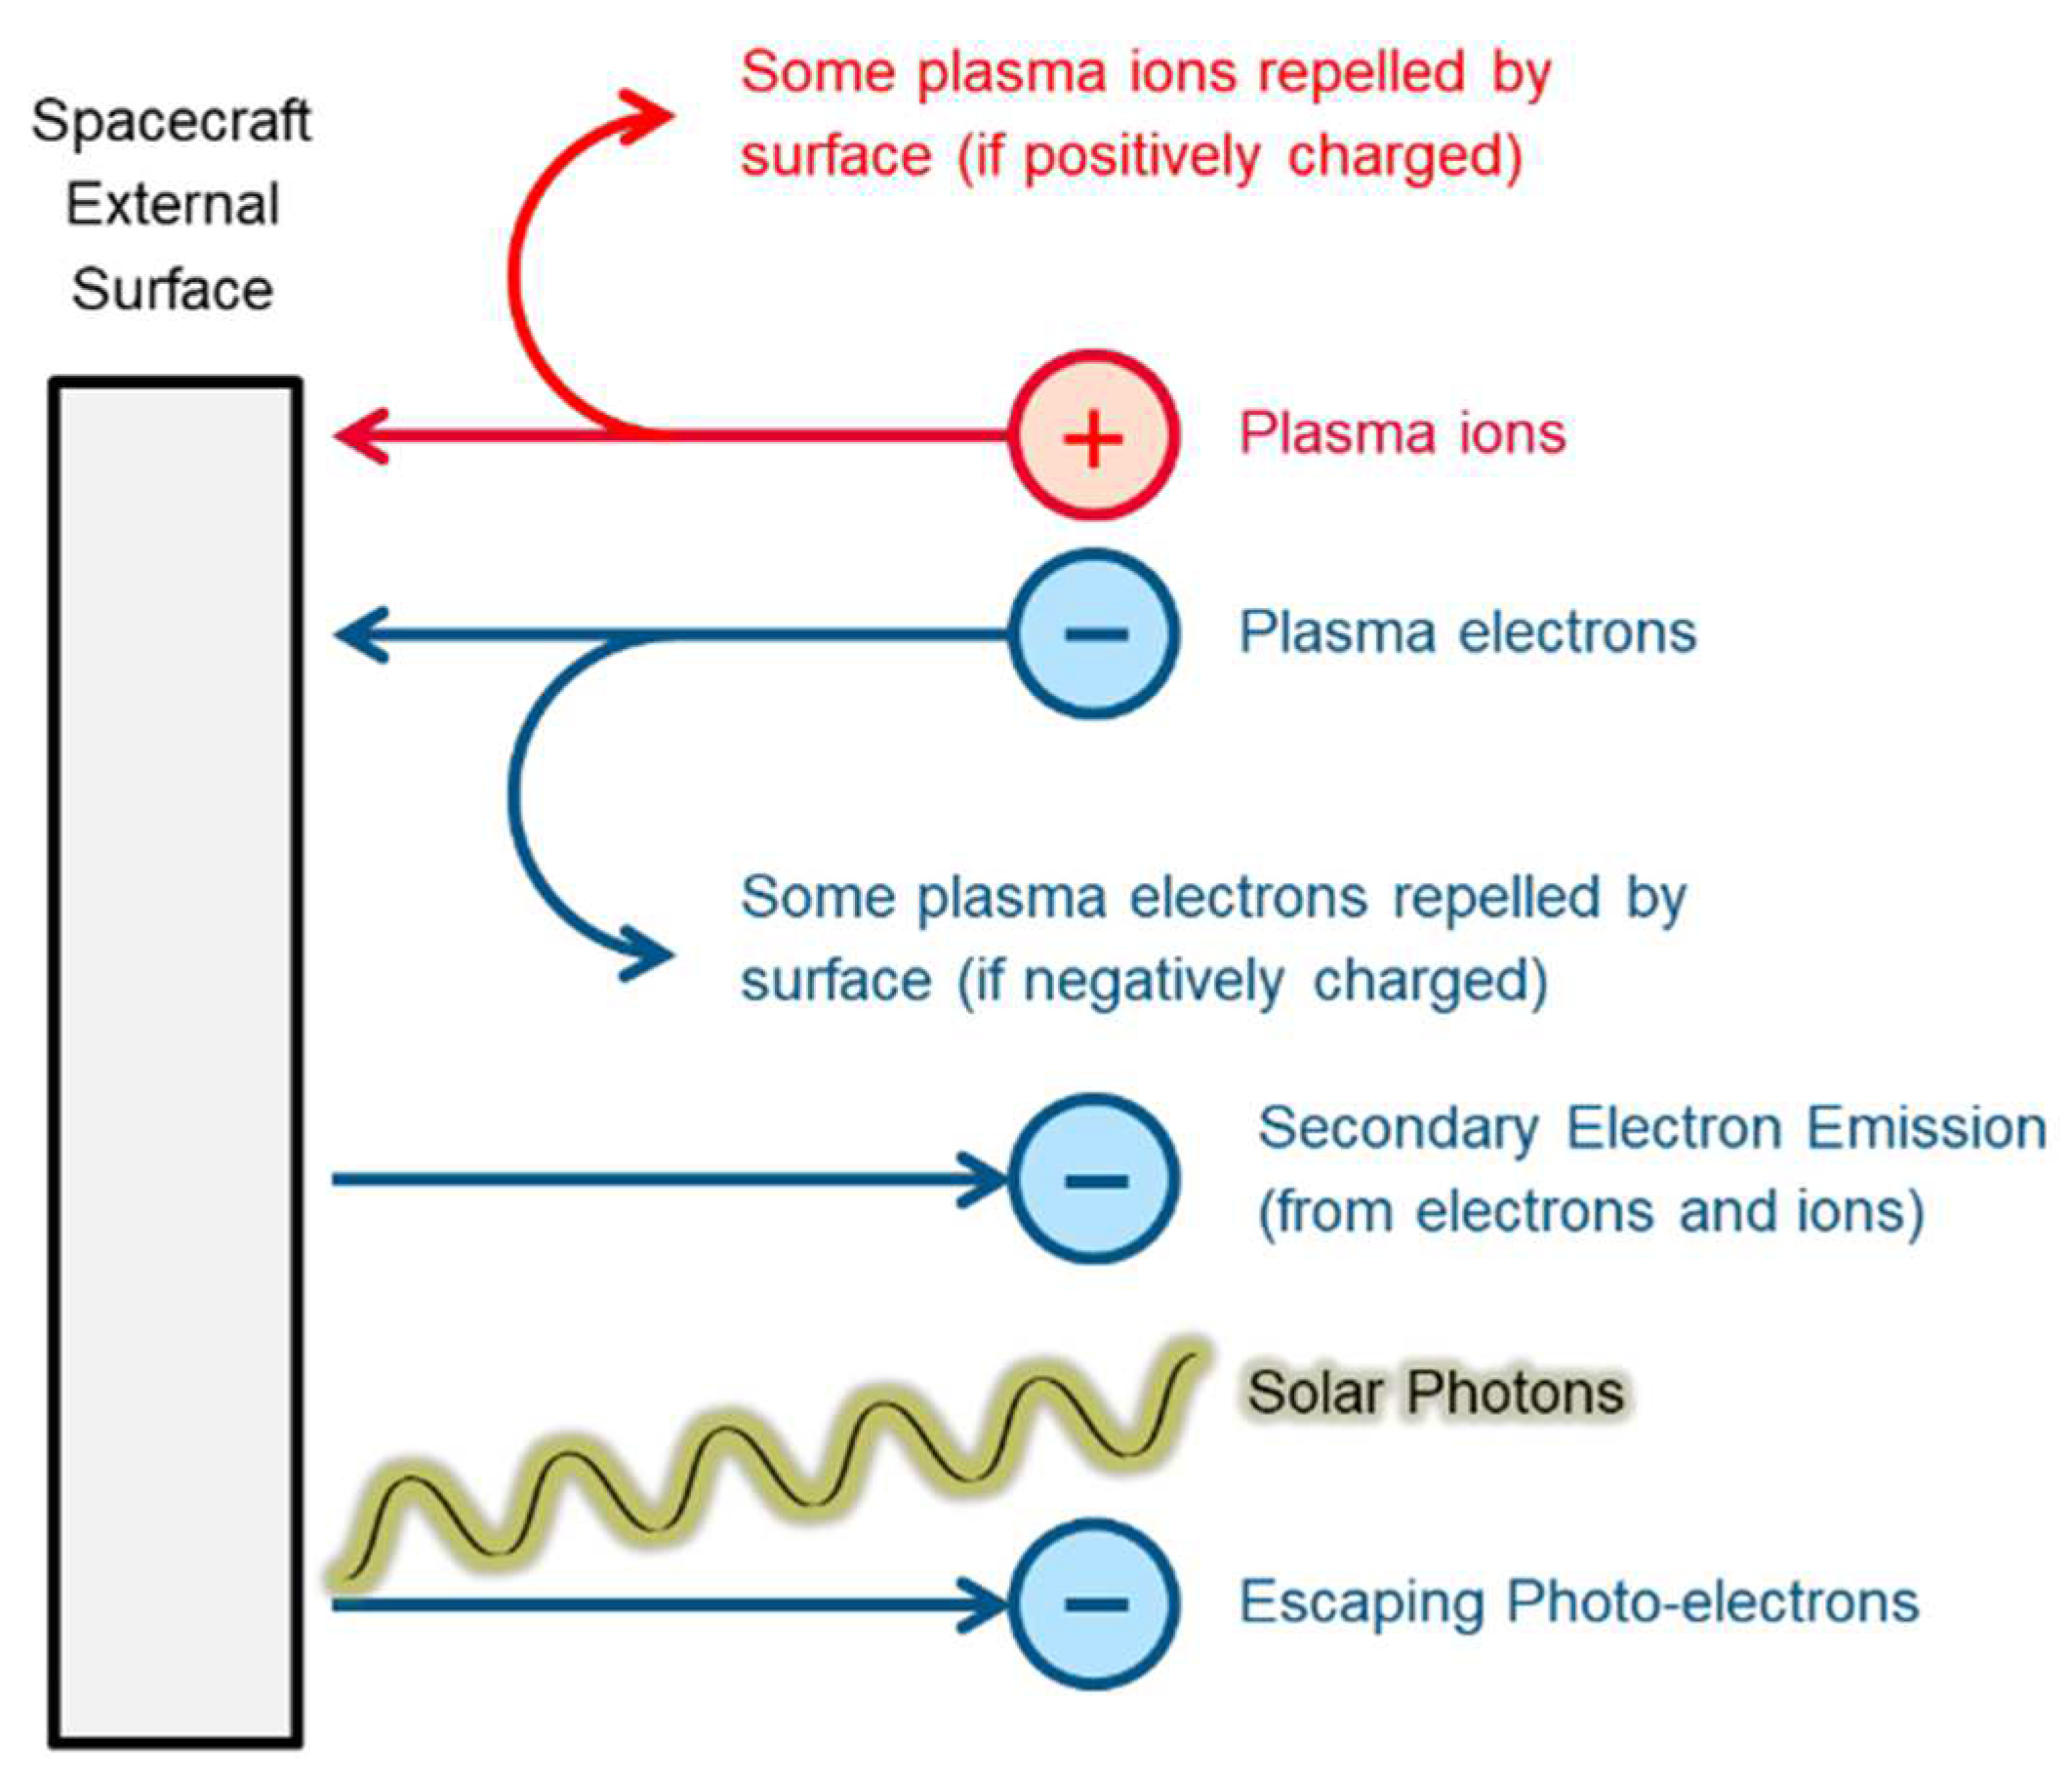
\includegraphics[width=.5\textwidth]{surface charging.png}
    \caption{Ariel spacecraft external surfaces' charging mechanism \protect\cite{Michelagnoli_Focardi_Pudney_Renouf_Merola_Noce_Nunez_Dinuzzi_Chiarucci_2024}.}
    \label{fig:10}  
\end{figure}

To assess charge distribution, simulations were conducted using a simplified CAD model of Ariel, developed with aid from AIRBUS Defense and Space. Due to the complexity of the spacecraft's materials, including Carbon Fiber-Reinforced Polymer, aluminium honeycomb structures, and 
advanced thermal cooling systems, the model was adjusted to optimise computational efficiency and to avoid overloading the Spacecraft Plasma Interaction System (SPIS) \cite{Michelagnoli_Focardi_Pudney_Renouf_Merola_Noce_Nunez_Dinuzzi_Chiarucci_2024}.
Simplifications of the structure included enlarging V-grooves, merging small surfaces, and representing the antenna as a single rod  (see Figure \ref{fig:12}).

\begin{figure}[H]
    \centering
    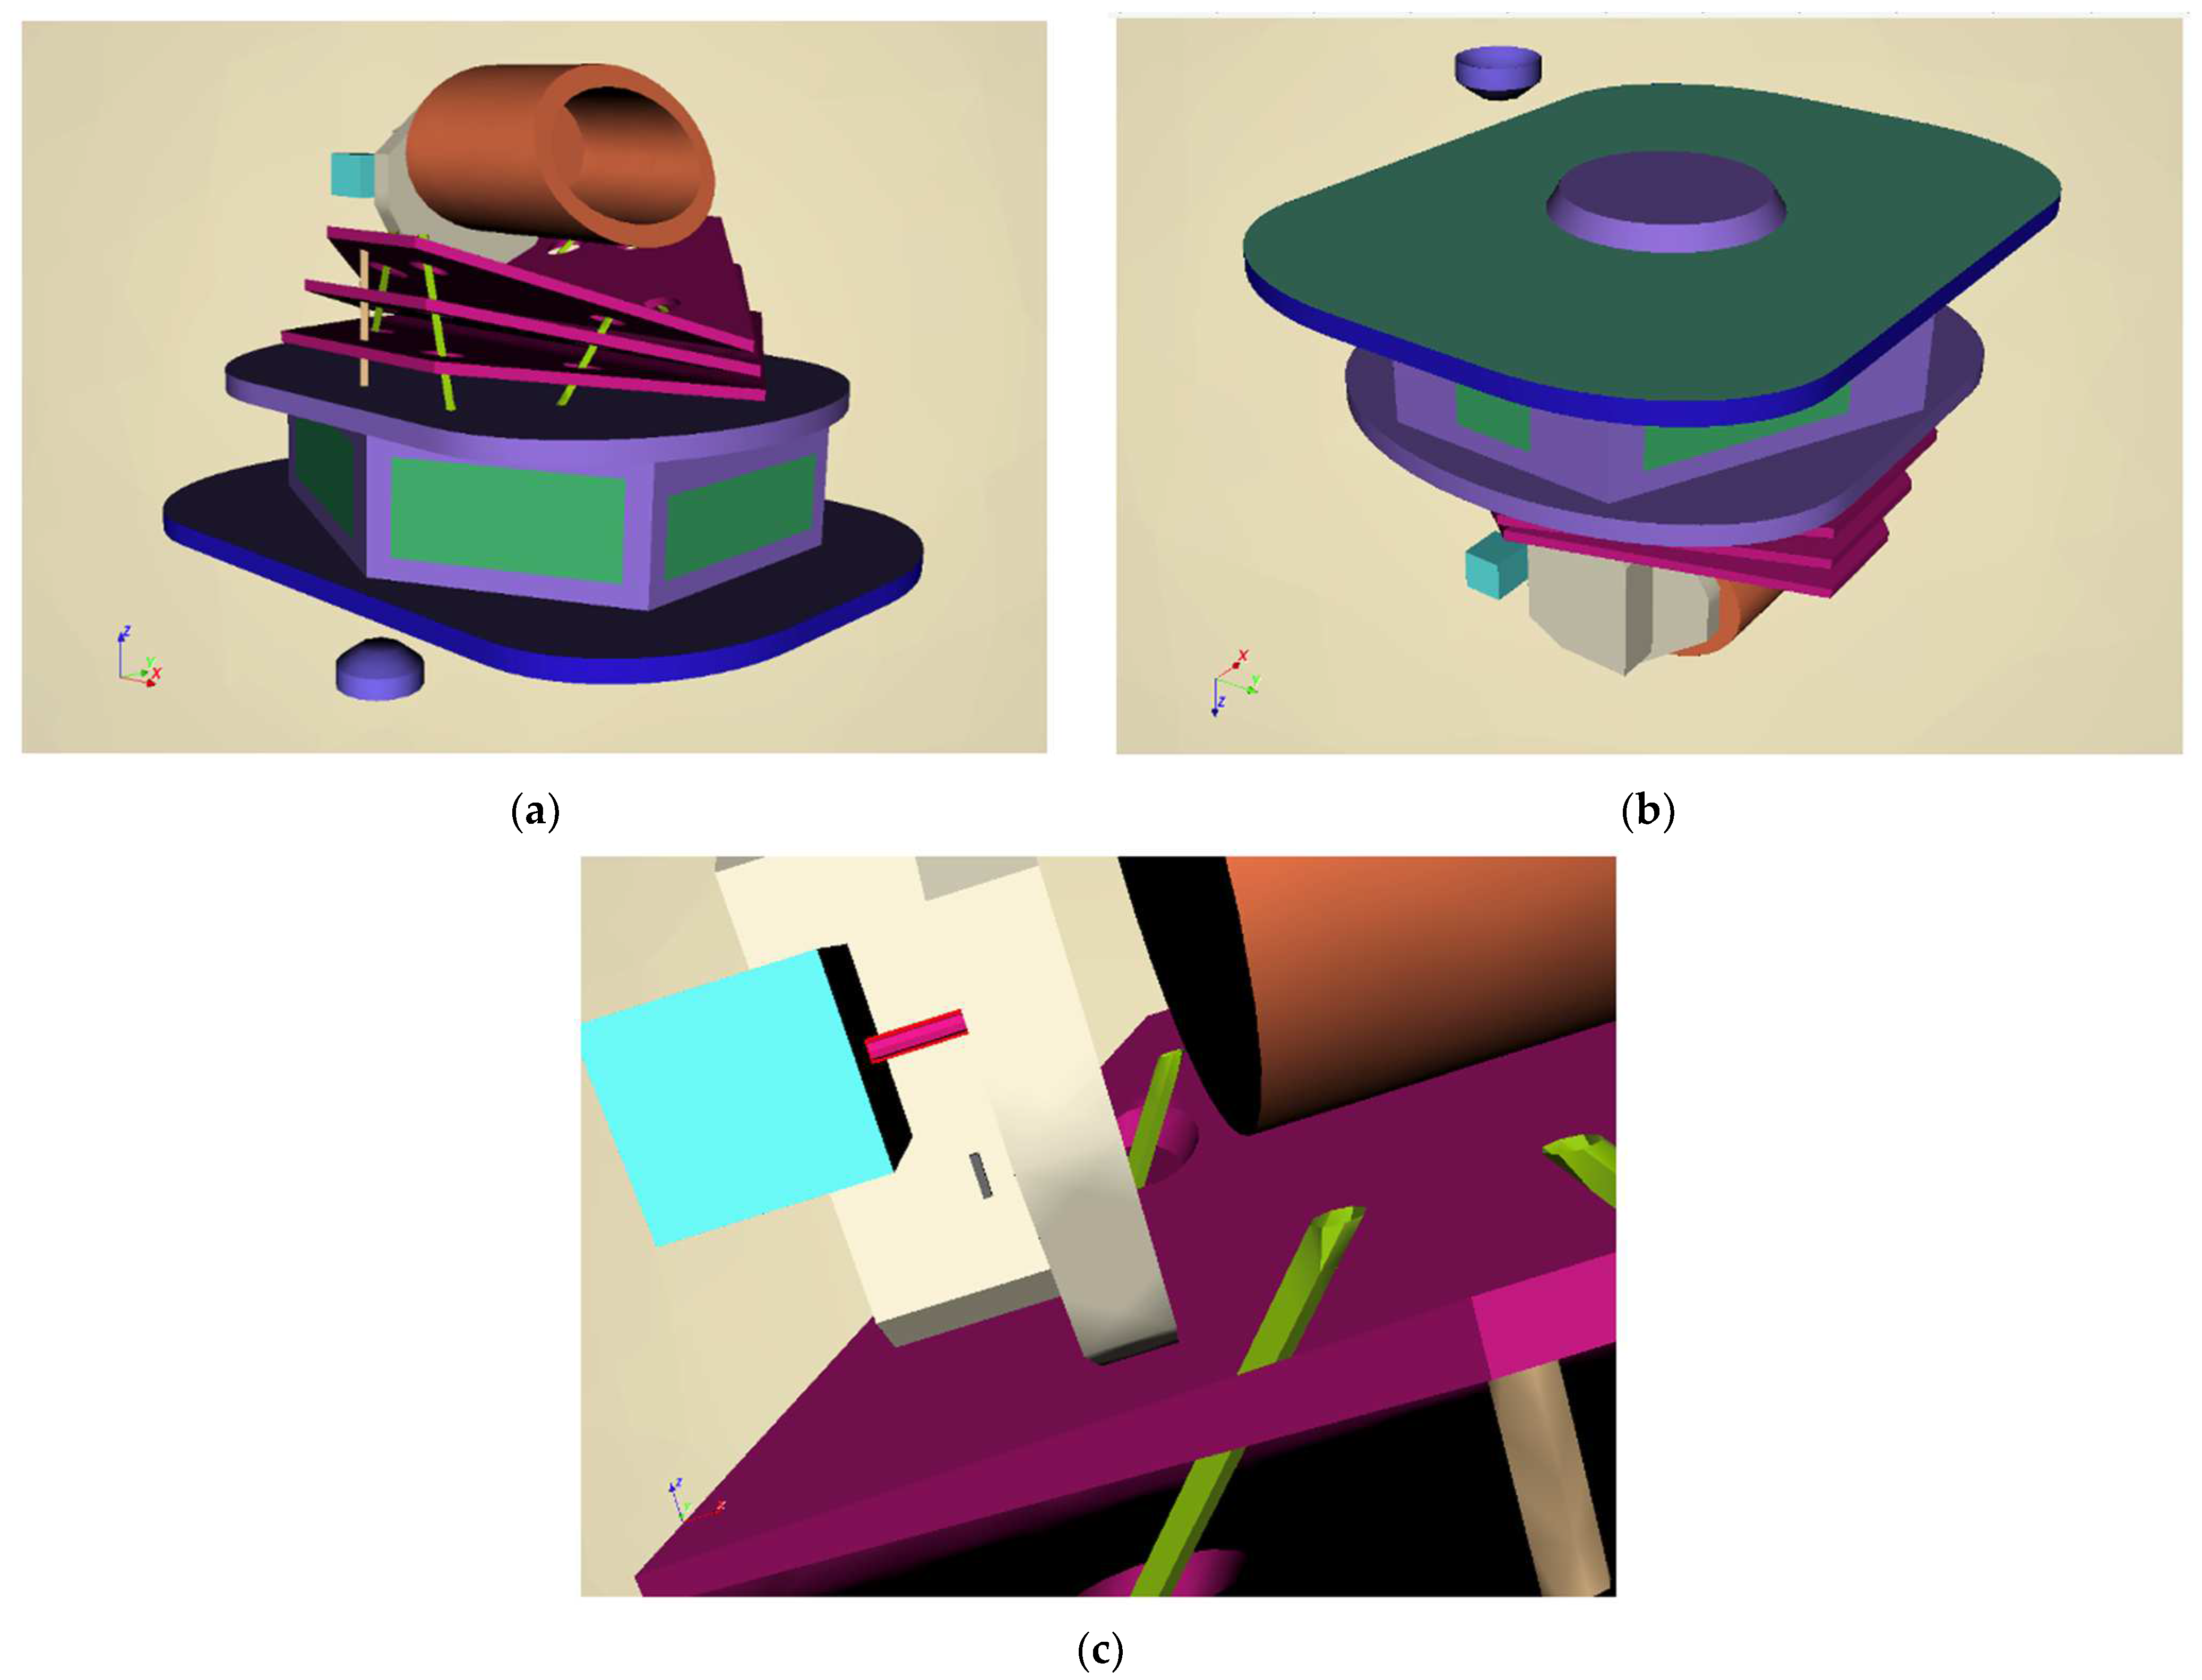
\includegraphics[width=.7\textwidth]{autoCAD ariel simple.png}
    \caption{Ariel geometrical model used for SPIS simulations: (a) front view; (b) bottom view; (c) close-up view of the FPE-IC connector and FPE strut \protect\cite{Michelagnoli_Focardi_Pudney_Renouf_Merola_Noce_Nunez_Dinuzzi_Chiarucci_2024}
    \newline (see Appendix for ESNs and allowed materials (\protect\ref{fig:13}); see Appendix for plasma parameters for SPIS simulations (\protect\ref{fig:14}))}
    \label{fig:12}
\end{figure}

Simulation results showed minimal charge accumulation at L2, with no significant risk. However, the GEO posed the greatest concern, with plasma interactions leading to differential charging. Within the magnetosheath, solar panels reached +14 V while payload struts charged to -7 V, which is within safe limits.
While charging disparities increased in some areas, only the GEO was identified as a danger zone. Suitable precautions have been taken, and critical equipment will be powered down during this phase \cite{Michelagnoli_Focardi_Pudney_Renouf_Merola_Noce_Nunez_Dinuzzi_Chiarucci_2024}.

\paragraph{Thermoelastic Analysis} ~\\

To ensure accurate results, the efficiency of Ariel's PLM must be maximised by analysing the thermal and structural effects on its performance. A STOP (Structural, Thermal, and Optical Performance analysis) was conducted, focusing on wavefront error and mirror
pointing accuracy, which are critical for data clarity and module optimisation \cite{Garcia-Perez_Alonso_Gomez-San-Juan_Perez-Alvarez_2021}.

The PLM experiences temperature variations and gravitational shifts after leaving Earth's orbit. To model these effects, a Finite Element Model (FEM) was employed, which is an industry-standard technique in aerospace engineering to examine the behaviour of the module under different load and temperature conditions \cite{Garcia-Perez_Alonso_Gomez-San-Juan_Perez-Alvarez_2021}.
Ariel's FEM, developed using NASTRAN code and refined from the JUICE mission, consists of 575 000 nodes, with key structural elements represented as tetrahedral parabolic elements of precision \cite{Garcia-Perez_Alonso_Gomez-San-Juan_Perez-Alvarez_2021}.

A crucial aspect of this analysis was defining the coefficient of thermal expansion (CTE) at cryogenic temperatures ($\sim$50 K). Using a reference temperature of 293 K, the equivalent equation for the CTE can be defined as \cite{Garcia-Perez_Alonso_Gomez-San-Juan_Perez-Alvarez_2021},

\vspace{-2ex}
\begin{gather*}
    CTE_{eq}(T) = \frac{\epsilon (T)}{T-T_{ref}} = \frac{\int^T_{T_{ref}} CTE(T) dt}{T-T_{ref}}
\end{gather*}

where $T_{ref}$ is the reference temperature and CTE(T) is the polynomial describing thermal expansion. Thermal strain ($\epsilon (T)$) is then expressed as,

\vspace{-2ex}
\begin{gather*}
    \epsilon (T) = [b(T-T_{ref}) + c(T^2 - T^2_{ref}) + d(T^3-T^3_{ref}) + e(T^4-T^4_{ref})] \times 10^{-5}
\end{gather*}

To ensure precision, the FEM simulations were compared with physical tests across various materials and temperatures. The primary source of error stemmed from joint modelling inaccuracies, leading to recommendations for refinement as module
specifications were finalised \cite{Garcia-Perez_Alonso_Gomez-San-Juan_Perez-Alvarez_2021}.

Tests were conducted for uniform and non-uniform temperature distributions, revealing quasi-homothetic deformations (symmetrical shifts) and rotations around the lateral axis. These displacements can be studied and the module can be altered accordingly \cite{Garcia-Perez_Alonso_Gomez-San-Juan_Perez-Alvarez_2021}.

\paragraph{Additional Planned Testing} ~\\

Several less significant but crucial tests will be conducted on Ariel's PLM.

\textbf{Radiometric calibration} will determine the ratio of detected signal to incident spectral power, providing direct stellar flux measurements essential for deriving planetary flux and radius from eclipse spectra. This involves applying known power levels and measuring focal length response across a range of wavelengths \cite{spry2023testing}.

The \textbf{system Figure of Merit} will be assessed to verify the payload's noise floor, ensuring Ariel operates within its photon noise limitations. \textbf{Spectral stray light} tests will also optimise power utilisation within the module \cite{spry2023testing}.

To maintain precision, \textbf{gain drift variation} tests will ensure Ariel's measurements remain stable within tens of ppm over 10-hour timescales, preventing artificial signal variations. Additionally, \textbf{Random Telegraph Signals (RTS)},
which cause discrete data jumps and potential errors, will be analysed and limited \cite{spry2023testing}.

\newpage

\section{Conclusion} \label{sec:5}

The Ariel mission represents a transformative step in exoplanet research, offering unprecedented spectroscopic data that will deepen the understanding of planetary formation, composition, and atmospheric processes. By systematically analysing
over 500 exoplanets in visible and infrared wavelengths, Ariel will provide a large-scale dataset that enables statistically significant comaprisons across diverse planetary environments.

Unlike past missions that were primarily focused on exoplanetary discovery, Ariel's targeted atmospheric Characterisation will reveal essential trends in planetary chemistry, thermal dynamics, and structural properties. These insights will refine the current models of 
planetary system evolution and contribute to the understanding of habitability conditions beyond the Solar System.

In unity with the JWST, ELT, and other observatories and telescopes, Ariel's findings will extend far beyond its operational lifetime, shaping the future of exoplanetary research. By addressing fundamental
questions about planetary diversity and origins, Ariel will not only enhance the knowledge of distant worlds but also offer critical context or understanding Earth's place in the universe.

\newpage

%%%%%%%%%%%%%%%%%%%%%%%%%%%%%%%%%%%

\bibliographystyle{IEEEtran}
\bibliography{References} \label{sec:ref}

\newpage

\section*{Contributions}
\addcontentsline{toc}{section}{Contributions}

Each team member has played a vital on the research and compilation of this report on the Ariel mission, ensuring a comprehensive and well-structured analysis.

\textbf{Joana Carranço Cabral Adão}

Compiled this report as a LaTeX document, edited various sections, and contributed to Tiers 1-3 (§\ref{sec:3.3.1}-§\ref{sec:3.3.3}), spacecraft details (§\ref{sec:4.2.3}-§\ref{sec:4.2.4}), and mission architecture (§\ref{sec:2}).

\textbf{Kyla Boyle}

Authored the section on the analysis and testing of the PLM (§\ref{sec:4.2.5}) and assisted with editing.

\textbf{Ewan Finlayson}

Contributed to the sections on the SVM (§\ref{sec:4.1}) and PLM (§\ref{sec:4.2}).

\textbf{Ananya Laxmeshwar}

Authored the motivation for the mission (§\ref{sec:1.1}, §\ref{sec:3.1}, §\ref{sec:3.4}) and assisted with editing.

\textbf{Isha Mathew}

Contributed to Tiers 2-4 (§\ref{sec:3.3.2}-§\ref{sec:3.3.4}) and mission architecture (§\ref{sec:2})

\textbf{Matilda Onnebrink}

Authored the introduction (§\ref{sec:1}) and the conclusion (§\ref{sec:5}).

\textbf{Brian Woods}

Contributed to spacecraft overview section (§\ref{sec:4}).

\section*{Appendix}
\addcontentsline{toc}{section}{Appendix}

\begin{figure}[H]
    \centering
    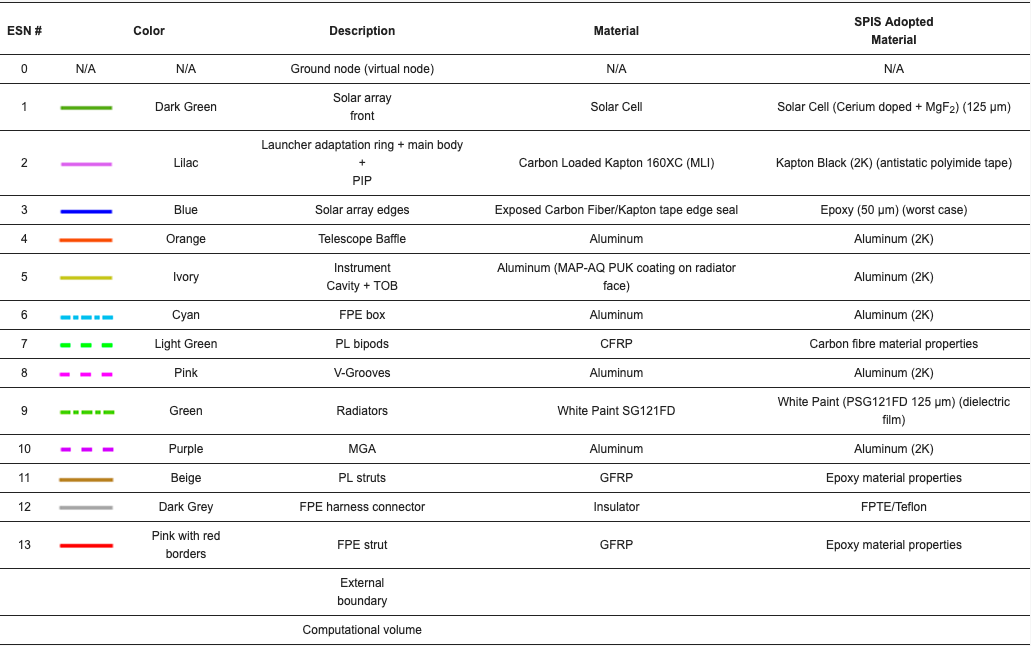
\includegraphics[width=\textwidth]{materials ariel autoCAD.png}
    \caption{\centering Table of ESNs (Electrical Super Nodes) and selected materials \protect\cite{Michelagnoli_Focardi_Pudney_Renouf_Merola_Noce_Nunez_Dinuzzi_Chiarucci_2024}.}
    \label{fig:13}
\end{figure}

\begin{figure}[H]
    \centering
    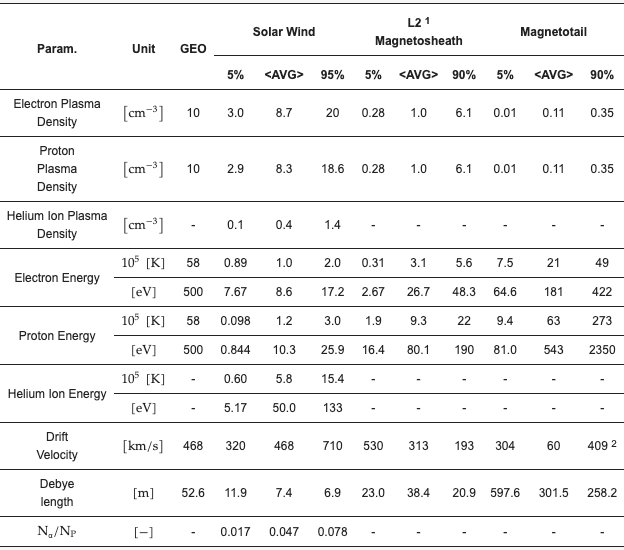
\includegraphics[width=.7\textwidth]{ariel plasma param.png}
    \caption{\centering Table of plasma parameters used for SPIS simulations \protect\cite{Michelagnoli_Focardi_Pudney_Renouf_Merola_Noce_Nunez_Dinuzzi_Chiarucci_2024}.}
    \label{fig:14}
\end{figure}

\listoffigures

\listoftables

\end{document}